% !TeX program = latexmk
% Chinese review manuscript; English master and submission source: dp_puzzle.tex.
% Engine and output directory are set by .latexmkrc (XeLaTeX, build/).
\RequirePackage[T1]{fontenc}
\documentclass[conference,10pt,letterpaper]{IEEEtran}
\usepackage[no-math]{fontspec}
\usepackage{xeCJK}
\setmainfont{TeX Gyre Termes}
\setsansfont{TeX Gyre Heros}
\setmonofont{TeX Gyre Cursor}
\setCJKmainfont{FandolSong-Regular.otf}[
  BoldFont=FandolSong-Bold.otf,
  ItalicFont=FandolKai-Regular.otf,
  SmallCapsFont=FandolSong-Regular.otf]
\setCJKsansfont{FandolHei-Regular.otf}[BoldFont=FandolHei-Bold.otf]
\setCJKmonofont{FandolFang-Regular.otf}
\usepackage{amsmath,amssymb}
\usepackage{graphicx}
\usepackage[caption=false,font=footnotesize]{subfig}
\usepackage{booktabs}
\usepackage{cite}
\usepackage[hidelinks]{hyperref}
\graphicspath{{figures/}}


\newcommand{\PaperTitle}{DP-Puzzle: Exploring Multi-Precision Throughput Ratios in Tensor Cores through Composable Dot-Product Units}
\title{\PaperTitle}
\author{\IEEEauthorblockN{Anonymous Submission}}
\hypersetup{
  pdfauthor={},
  pdftitle={\PaperTitle},
  pdfsubject={Chinese working draft}}

\newcounter{DACreferencepage}
\AtEndDocument{%
  \ifnum\value{page}>\value{DACreferencepage}\relax
    \PackageWarningNoLine{DAC2027}{References exceed one page}%
  \fi}

\begin{document}
\bstctlcite{DPBSTcontrol}
\maketitle

% !TeX root = ../main.tex
\begin{abstract}
MXFP8和MXFP4等微缩格式在大型语言模型中得到了更广泛的应用。这一趋势推动了对基于点积的张量核中增加低精度算力的需求。然而，不同多精度算力配比的硬件成本和工作负载效益缺乏系统性的评估。为了填补这一空白，我们提出了DP-Puzzle，这是一个基于可组合点积单元的设计空间探索框架。这些单元在不同精度之间共享计算数据路径，并包含专用的低精度扩展以支持不同的峰值算力配比。该框架将电路级面积和功耗特性与当前工作负载和潜在精度偏移的模型相结合。在计算核心的总面积预算固定的情况下，DP-Puzzle评估了候选设计的计算延迟和能耗。这一分析为硅前芯片设计期间基于工作负载的算力配比选择提供了量化依据。

\end{abstract}
\begin{IEEEkeywords}
设计空间探索，多精度算力配比，组合式点积单元，张量计算，硬件成本建模
\end{IEEEkeywords}


% !TeX root = ../main.tex
\section{引言}
\label{sec:introduction}
随着 AI 模型规模与计算需求的增长，低精度浮点计算正成为提升计算效率的重要途径，FP8 及更低位宽格式已逐步用于实际模型。DeepSeek-V3 在混合精度训练中以 FP8 执行主要线性层的前向与反向矩阵乘法~\cite{deepseekv3}；GLM-4.5 在保留 BF16 参数更新的同时，通过在线 FP8 量化加速强化学习中的采样推理~\cite{glm45}。面向更低位宽，DeepSeek-V4 通过量化感知训练将 MoE 专家权重量化为 MXFP4 用于部署，并在长上下文注意力索引器中以 MXFP4 存储 Q/K 激活、执行点积计算~\cite{deepseekv4}。这些实践表明，低精度需求已从 FP8 矩阵计算进一步扩展至 FP4 计算与存储。与此同时，模型各部分对数值误差的容忍程度不同，输出层、注意力等敏感计算仍需保留 BF16 等较高精度的矩阵运算~\cite{deepseekv3}。因此，实际负载对张量计算硬件提出了多种精度并存的需求。但是，从低精度浮点本身特性来看，低位宽能够减少数据存储与搬运开销，并为在有限硬件资源下提高计算并行度提供空间，成为未来AI模型计算精度选择的一个重要方向。而在面积与功耗预算约束下，如何兼顾较高精度计算能力与低精度吞吐需求，进而确定 16、8、4 位浮点张量计算的峰值算力配比，也成为当前乃至未来AI芯片的重要架构设计问题。

当前产业界的配比选择已呈现多样化趋势。以同一芯片的 16 位峰值算力归一化，按各精度稠密矩阵计算峰值比较，NVIDIA B200、AMD MI355X 与华为 Ascend 950PR 采用经典的 $1:2:4$ 配比~\cite{nvidiahgx,amdmi355x,huawei950}；NVIDIA B300 将配比调整为 $1:2:6$~\cite{nvidiahgx}，AMD MI455X 约为 $1:4:8$~\cite{amdmi455x}，华为 Ascend 960PR 的公开研发路线目标则为 $1:2:8$~\cite{huawei960roadmap}。从硬件规划的角度看，低精度算力增配具有面向未来负载的前瞻性。芯片从架构设计、验证到流片部署需要较长周期，而模型结构与量化方法迭代更快；设计阶段观察到的精度需求，未必能代表芯片部署及使用期间的负载。因此，配比选择需要预估未来低精度计算需求的增长，在芯片设计阶段提前配置相应资源。

然而，公开规格展示了配比选择的结果，却不足以说明这些配比如何实现，以及新增的面积、功耗与带宽需求能够换来多少可用算力。即使配比相同，不同的归约长度、输出并行度与后端共享范围，也会改变资源开销及算力发挥所需的数据供给条件。现有多精度计算与设计空间探索研究已考察通路复用、数值格式及硬件成本之间的关系~\cite{transdot2026,paretomac2025,zhao2026mxlike}，但面向算力配比及其实现方式，仍缺少可复现、可对比的系统评估。面向尚未确定的未来负载，需要将配比、实现方式与资源约束纳入统一框架，考察不同精度需求下的成本与算力收益，为前瞻性配比选择提供依据。

为此，本文提出 DP-Puzzle，一种面向多精度浮点张量计算的分层可组合点积架构。在点积单元（dot-product unit）内部，通过跨精度资源复用与低精度专用计算模块的组合，沿归约维度 $K$ 增加目标精度下每周期处理的乘积项数；在阵列层面，通过组合具有不同精度支持与计算能力的点积单元，沿输出维度 $N$ 调整各精度下的输出并行度。两类组合分别在单元内部与阵列层面改变算力配比。在给定 Tensor Core 或阵列面积预算下，本文结合面积、功耗与带宽模型，比较两类实现，并分析不同精度负载及数据供给条件下的算力收益与帕累托权衡，为未来芯片的配比规划提供可比较的硬件实现与成本依据。

本文的主要贡献如下：

\begin{enumerate}
  \item \textbf{支持多精度浮点精度的点积单元设计。} 结合新型浮点精度格式定义，通过合理设计分组，针对乘法器，加法器与移位器资源复用，支持BF16、FP16、MXFP8/6/4、NVFP4与HiF4等多精度浮点计算。
  \item \textbf{提出两种改变传统配比的实现方式，并进行硬件成本与收益分析。} 在匹配各精度绝对计算能力的条件下，对比单元内 $K$ 向组合与阵列级 $N$ 向组合的面积、功耗与带宽成本。在所评估配置中，单元内 $K$ 向扩展具有面积优势，能耗收益则与目标精度和阵列规模有关；两类组合的带宽需求增长随阵列输出维规模而变化。
  \item \textbf{建立负载驱动的配比选择方法。} 针对四种代表配比，建立固定整核面积、整数部署和混合精度时间／能耗模型，以精确选择边界连接硬件成本与真实模型结构导出的 prefill 工作量，揭示配比收益随上下文和执行精度变化的规律。
\end{enumerate}

本文其余部分安排如下：第~\ref{sec:background} 节介绍背景与相关工作；第~\ref{sec:architecture} 节说明 DP-Puzzle 架构及配比实现方法；第~\ref{sec:evaluation} 节评估组合成本与配比收益；第~\ref{sec:conclusion} 节总结全文。


% !TeX root = ../main.tex
\section{背景与动机}
\label{sec:background}

\subsection{浮点精度与微缩放格式}
\label{sec:formats}

BF16/FP16 由逐元素的指数与有效数确定动态范围和精度~\cite{burgess2019bfloat16}；微缩放格式则将低位宽元素与共享尺度共同编码（图~\ref{fig:fpformats}）。OCP MXFP8/6/4 采用 32 元素一组的 E8M0 尺度~\cite{ocpmx2023}；NVFP4 使用 16 元素一组的 E4M3 尺度~\cite{nvidia2024nvfp4}；HiF4 使用 64 元素一组的无符号 E6M2 基础尺度，并为每 8、4 个元素分别配置一位微指数~\cite{hifloat4}。元素编码、分组粒度和尺度编码分别决定解包、局部规约与尺度融合的硬件需求。

\begin{figure}[t]
\centering
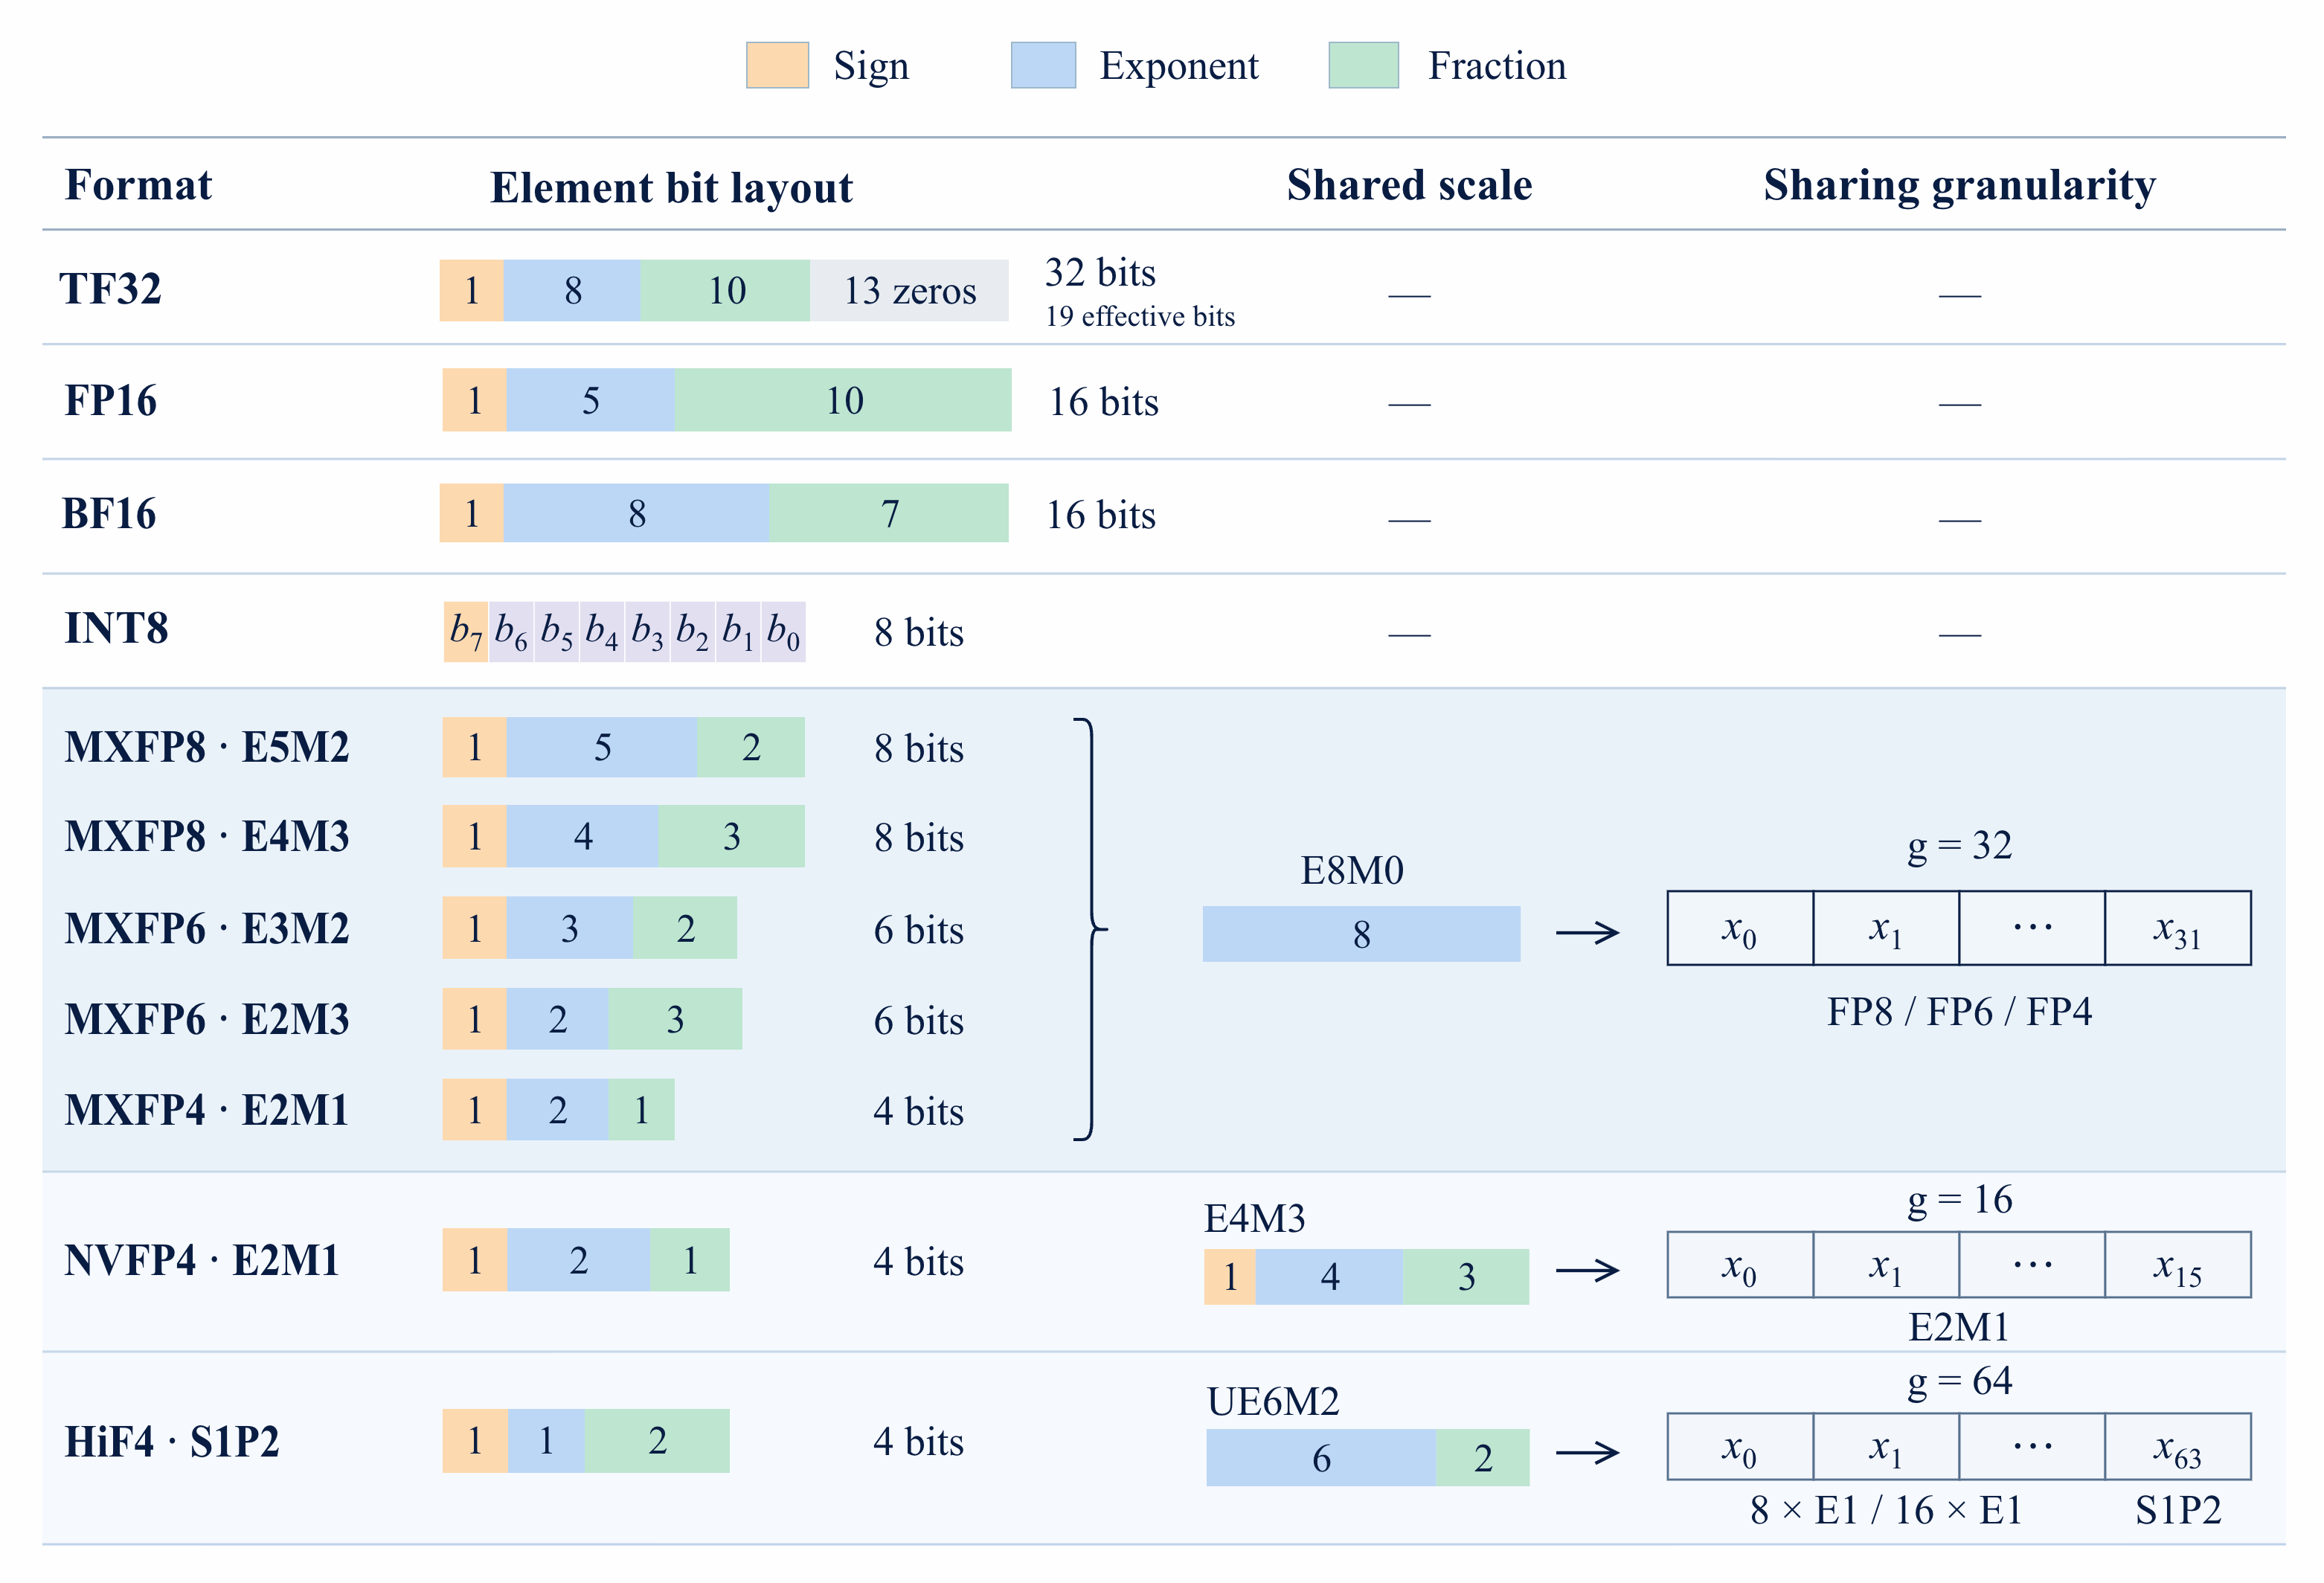
\includegraphics[width=\columnwidth]{fp_format.png}
\caption{元素编码与共享尺度~\cite{ocpmx2023,nvidia2024nvfp4,hifloat4}。字段标注为位宽，$g$ 为缩放组大小。}
\label{fig:fpformats}
\end{figure}


\subsection{张量计算与点积单元}
\label{sec:tensor_organization}

对于矩阵乘累加 $D=C+AB$，$M$、$N$ 是输出维度，$K$ 是归约维度。点积单元先对齐多个乘积并集中归约，再统一规格化和舍入，以共享后端摊薄逐项浮点处理的成本~\cite{lutzFusedFP84Way2024}。本文采用 H 类原生归约长度为 16 的 DP 作为基线，与已有数值建模研究识别的点积累加粒度相对应~\cite{xie2025mmasim}。完整 GEMM 沿归约维拆为多笔请求，单 DP 接收显式 $C$ 并输出 $D$，跨请求部分和保存在其外部。

有无组尺度的格式可用同一局部点积结构描述。依据 OCP 的点积定义，共享尺度可提出组内归约~\cite{ocpmx2023}。将 $L$ 项乘积按缩放组边界划分为 $G=\lceil L/g\rceil$ 组，末组不足部分补零，加入累加输入 $c$ 后，有
\begin{equation}
d=c+\sum_{j=0}^{G-1}X_j^{(A)}X_j^{(B)}
\underbrace{\sum_{i=0}^{g-1}P_{j,i}^{(A)}P_{j,i}^{(B)}}_{q_j}.
\label{eq:blockdot}
\end{equation}
其中，$X_j^{(A)}$、$X_j^{(B)}$ 为两路输入第 $j$ 组的共享尺度，$P_{j,i}^{(A)}$、$P_{j,i}^{(B)}$ 为组内元素的解码值，$q_j$ 为组内点积；HiF4 的局部微指数计入元素解码。对于无组尺度的格式，令 $X_j^{(A)}=X_j^{(B)}=1$，即可得到普通点积累加。

式~\eqref{eq:blockdot} 给出分层共享的算术边界；内部位宽、顺序与舍入仍由具体实现约束。



\subsection{通路复用与设计空间探索}
\label{sec:datapath_sharing}

表~\ref{tab:related_features} 汇总格式与组合能力。MX 列区分完整微缩放支持与仅元素运算支持；本文通过在共享 DP 内增配专用 Group 改变算力配比。

% Entries refer to reported configurations, not hypothetical reconfiguration.
\begin{table*}[t]
\centering
\caption{Supported input formats and datapath features of related arithmetic units.}
\label{tab:related_features}
\begingroup\footnotesize\setlength{\tabcolsep}{3pt}
\def\Y{$\checkmark$}\def\N{$\times$}
\begin{tabular*}{\textwidth}{@{\extracolsep{\fill}}l*{14}{c}@{}}\toprule
& \multicolumn{9}{c}{Native input formats} & \multicolumn{5}{c}{Datapath features} \\
\cmidrule(lr){2-10}\cmidrule(lr){11-15}
Design & TF32 & FP16 & BF16 & FP8 & FP6 & FP4 & INT8 & INT4 & LOG4 & DP & MX & NVFP4 & HiF4 & SR \\\midrule
Ten-Four~\cite{rout2026tenfourv2} & \Y & \Y & \Y & \Y & \N & \N & \Y & \Y & \N & \Y & \Y & \N & \N & \N \\
MPICC~\cite{huangMPICCMultiplePrecisionInterCombined2025} & \N & \N & \N & \Y & \Y & \Y & \N & \Y & \Y & \Y & --- & \N & \N & \Y \\
MXDOTP~\cite{islamoglu2025mxdotp} & \N & \N & \N & \Y & \N & \N & \N & \N & \N & \Y & \Y & \N & \N & --- \\
FPnew~\cite{mach2020fpnew} & \N & \Y & \Y & \Y & \N & \N & \N & \N & \N & \N & \N & \N & \N & \N \\
TransDot~\cite{transdot2026} & \N & \Y & \N & \Y & \N & \Y & \N & \N & \N & \Y & \N & \N & \N & --- \\
\midrule
DP-Puzzle & \Y & \Y & \Y & \Y & \Y & \Y & \Y & \N & \N & \Y & \Y & \Y & \Y & \N \\
\bottomrule\end{tabular*}
\par\smallskip
\parbox{\textwidth}{\raggedright
$\checkmark$: supported; $\times$: absent from the reported configuration; ---: not established by the cited evidence.
DP: native multi-term dot product; MX/NVFP4/HiF4: integrated block-scale handling (MX indicates at least one MX format); SR: stochastic rounding.
FP8/FP4 denote element arithmetic and do not imply scale support. FPnew additionally supports FP32/64; TransDot supports FP32 FMA. MPICC supports heterogeneous operand combinations and FP12 emulation, which is not marked as native FP16.}
\endgroup
\end{table*}


已有工作通过跨精度共享降低单元成本：TransDot 重组乘法器与移位器~\cite{transdot2026}，MPICC 将多种格式映射为统一内部表示~\cite{huangMPICCMultiplePrecisionInterCombined2025}，融合 FP8 点积设计复用累加和舍入后端~\cite{lutzFusedFP84Way2024}。DSE 研究进一步联合探索数值格式与 MAC 微架构~\cite{paretomac2025}，或共享尺度、权重和激活格式~\cite{zhao2026mxlike}；Timeloop 则以循环分块与存储层次分析阵列映射~\cite{timeloop2019}。本文固定目标格式集合，将 H/Q/E 峰值配比作为设计变量，考察实测单元成本如何影响面积预算下的部署规模与负载收益。

\subsection{算力配比的设计动机}
\label{sec:commercial_ratios}
\label{sec:ratio_motivation}

表~\ref{tab:vendor_ratios} 给出代表性产品与研发路线的配比。本文选取 $1:2:4$、$1:2:6$、$1:2:8$ 和 $1:4:8$ 构成离散设计空间；这些数字仅规定各精度相对峰值，不预设面积或功耗按同一比例缩放。

\begin{table}[t]
\centering
\caption{各产品的稠密矩阵峰值（PFLOP/s）及研发路线目标。}
\label{tab:vendor_ratios}
\begingroup\footnotesize\setlength{\tabcolsep}{3pt}
\begin{tabular*}{\columnwidth}{@{\extracolsep{\fill}}lrrrl@{}}\toprule
Product & 16-bit & 8-bit & 4-bit & Ratio \\\midrule
B200 SXM~\cite{nvidiahgx} & 2.250 & 4.500 & 9.000 & $1:2:4$ \\
MI355X~\cite{amdmi355x} & 2.517 & 5.033 & 10.066 & $1:2:4$ \\
Ascend 950PR~\cite{huawei950} & 0.432 & 0.865 & 1.730 & $1:2:4$ \\
\midrule
B300 SXM~\cite{nvidiahgx} & 2.250 & 4.500 & 13.500 & $1:2:6$ \\
\midrule
Rubin GPU~\cite{nvidiaverarubin} & 4.000 & 17.500 & 35.000 & $\approx 1:4:8$ \\
MI455X~\cite{amdmi455x} & 5.033 & 20.133 & 40.265 & $1:4:8$ \\
\midrule
Ascend 960PR$^\dagger$~\cite{huawei960roadmap} & 1.000 & 2.000 & 8.000 & $1:2:8$ \\
\bottomrule
\end{tabular*}
\par\smallskip
\parbox{\columnwidth}{\raggedright 产品行使用稠密矩阵峰值；$\dagger$ 表示研发路线目标。}
\endgroup
\end{table}

配比选择包含两个相互关联的问题：增加低精度算力需要多少硬件资源，以及新增资源在给定工作量组成下能否缩短计算时间、降低能耗。前者需要可组合微架构及同工况成本表征；后者需要将面积引起的部署密度变化纳入负载模型。第~\ref{sec:architecture} 节构建候选 DP，第~\ref{sec:evaluation} 节表征其成本，第~\ref{sec:workload} 节在统一面积预算下分析配比的适用区域。


% !TeX root = ../main.tex
% 中文精简审核稿：经作者确认后再同步 dp_puzzle.tex；当前中英文差异为有意保留。
\section{共享多精度点积微架构}
\label{sec:architecture}
\label{sec:brick_definition}

DP-Puzzle 采用 Lane、Group 和 DP（dot-product unit）三层结构（图~\ref{fig:dp_architecture}）。Lane 复用元素乘法与局部对齐，Group 融合尺度并统一部分和表示，DP 共享全局对齐与累加后端。统一的 Group 接口使低精度前端能够独立裁剪和增配，是后续配比扩展的组合边界。

H、Q、E 分别覆盖 FP16/BF16、MXFP8/6 和 MXFP4/NVFP4/HiF4，T、I 分别表示 TF32 和 INT8。一个 Lane 支持 T1H2I4Q4E8，数字表示每拍处理的元素对数。两个 Lane 构成 Group，四个 Group 构成 T8H16I32Q32E64 基线。该层级覆盖 HiF4 的局部微指数与 NVFP4 的组尺度粒度，更大尺度块通过广播共享尺度。各模式采用八级流水，每拍接收一笔独立请求。

\begin{figure}[t]
\centering
\includegraphics[width=\columnwidth]{baseline_arch.png}
\caption{Lane--Group--DP 分层架构。Lane 共享乘法与局部移位，Group 完成尺度融合与指数重计算，DP 共享全局对齐及累加；整数模式旁路浮点对齐与输出处理。}
\label{fig:dp_architecture}
\end{figure}

\subsection{Lane：解码与算术复用}
\label{sec:unpack_recode}
\label{sec:full_brick}

图~\ref{fig:data_unpack} 给出共享计算所需的解包表示：T/H 保留指数与有效数，Q 统一为内部 E5M3 表示，INT8 分离符号与幅值。MXFP4/NVFP4 将元素指数融入 U3P1 定点幅值；HiF4 将一级微指数并入 U2P2 幅值，保留 Lane 共享的二级微指数。E 类因此无需逐元素浮点对齐。

\begin{figure}[t]
\centering
% 图稿待作者统一数量标签：按完整 Lane 标注时，FP16 为 2x，E 为 8x；
% 右侧 10/16/4 位描述单个字段组，每个 Lane 包含两个字段组。
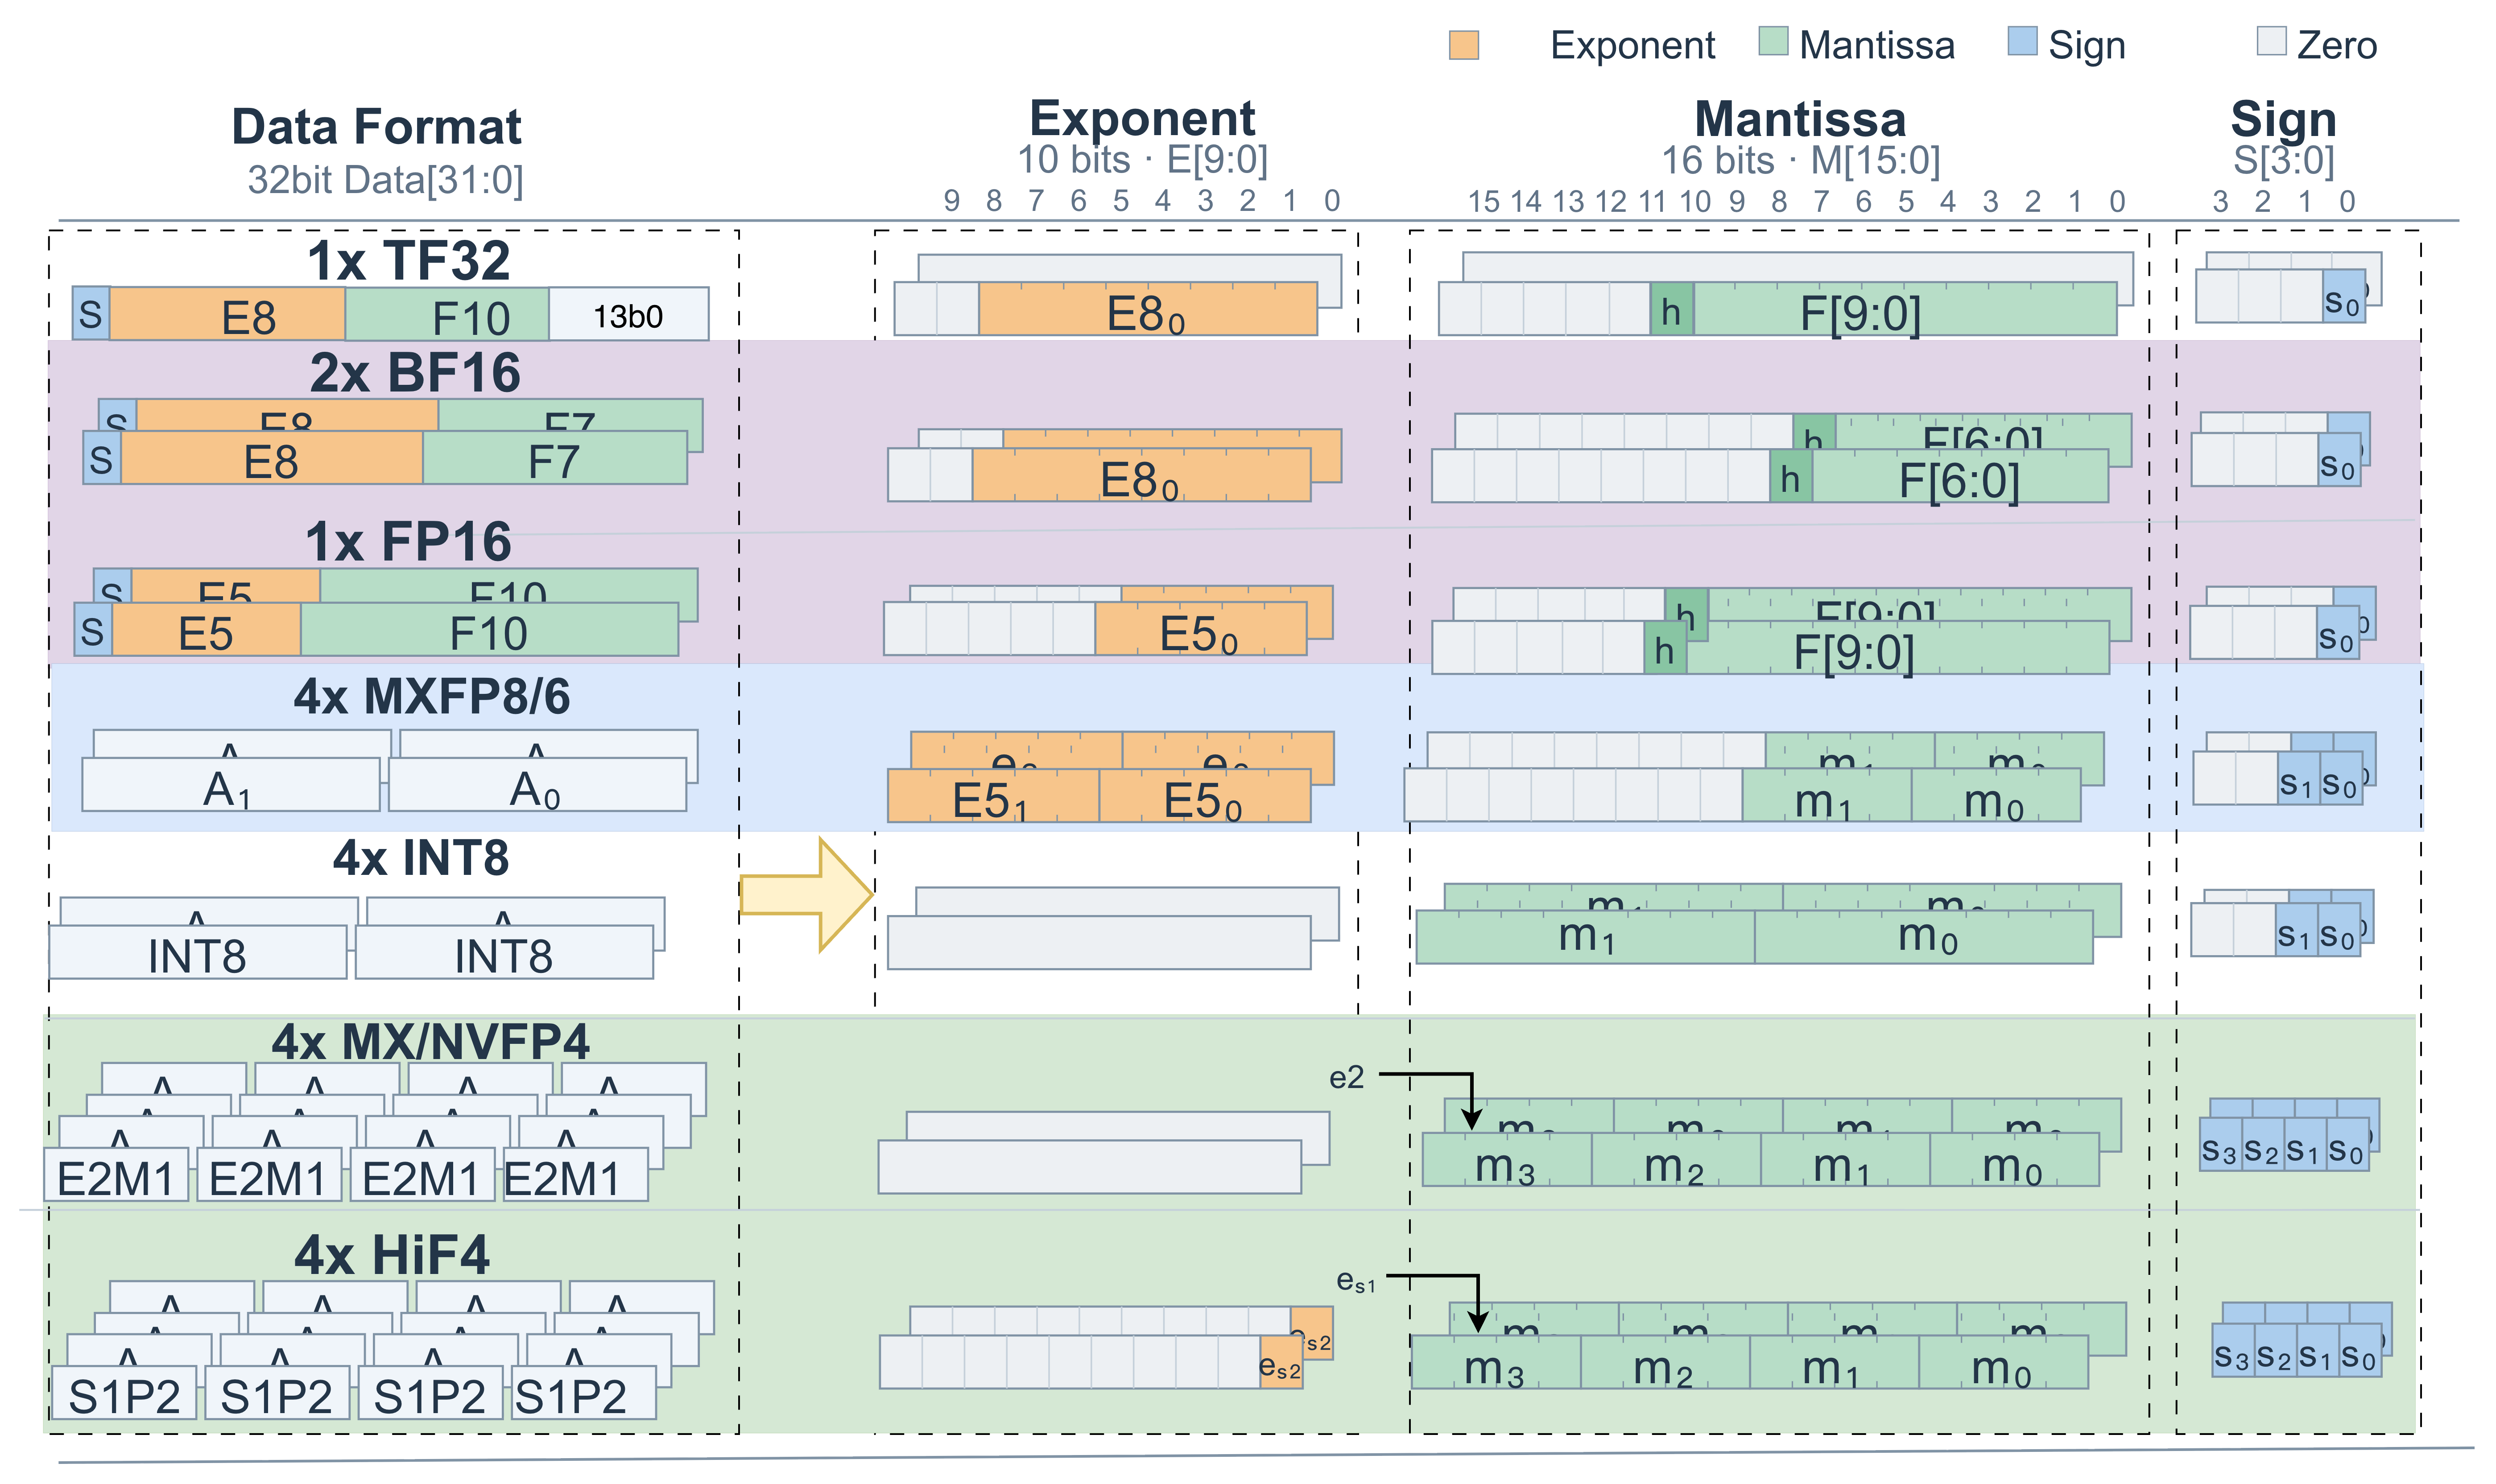
\includegraphics[width=\columnwidth]{unpack_layout.png}
\caption{输入格式到共享指数、有效数和符号字段的映射。Q 使用统一内部编码，E 将元素指数吸收到定点幅值中；未用字段补零，特殊值标志独立传播。}
\label{fig:data_unpack}
\end{figure}

\textbf{乘法器复用。}Ten-Four 按有效数位宽类别共享乘法器~\cite{rout2026tenfourv2}。本文采用两套 $8\times8$、$8\times4$、$4\times8$ 和 $4\times4$ 乘法单元，通过组合部分积支持宽乘法，通过独立路由支持多路低精度乘法，避免按格式复制完整乘法阵列。

\textbf{移位器复用。}T/H/Q 乘积按小数点位置静态补零后，进入四路共享右移器；本文选择 28\,bit 无符号局部对齐窗口。两个 Lane 使用共同的最大乘积指数完成对齐。E/INT8 旁路该网络，复用后续规约树；HiF4 在 Lane 部分和上施加二级微指数的小范围左移。

\subsection{Group：尺度融合与 Anchor Recompute}

\textbf{规约后尺度融合。}两个 Lane 共享尺度，Group 因而先求和并取幅值，再乘两侧尺度尾数的乘积 $\mathrm{Scale}_{\mathrm{mant}}$。NVFP4/HiF4 的紧凑组幅值为 U14，尺度尾数乘积为 U8，两种格式共用一套 U14$\times$U8 乘法器，避免逐元素复制尺度乘法。MX 的幂次尺度仅计入指数，旁路尾数乘法。

\textbf{统一部分和表示。}将 Group 输出幅值记为 $\mathrm{SoP}$（sum of products），位宽及小数位数分别记为 $\mathrm{Group}_{\mathrm{mag}}$ 和 $\mathrm{Group}_{\mathrm{frac}}$；本文采用 31\,bit 幅值。$\mathrm{Anchor}$ 表示幅值最高物理位对应的指数，由局部对齐指数 $\mathrm{Anchor}_{\mathrm{lane}}$、两侧尺度的无偏指数和 $\mathrm{Scale}_{\mathrm{exp}}$ 及元素偏置 $\mathrm{Bias}$ 共同确定：
\begin{equation}
\begin{aligned}
\mathrm{Anchor}={}&\mathrm{Anchor}_{\mathrm{lane}}+\mathrm{Scale}_{\mathrm{exp}}\\
 &+\mathrm{Group}_{\mathrm{mag}}-1-\mathrm{Group}_{\mathrm{frac}}-2\mathrm{Bias}.
\end{aligned}
\label{eq:anchor_recompute}
\end{equation}
格式相关修正可预先确定，使 Anchor Recompute 与尾数规约并行。E 的元素指数已融入幅值，局部对齐指数与元素偏置均取零；无尺度格式的尺度指数和取零。

\textbf{前导零与双向移位。}Group 在尺度融合后的 SoP 上检测前导零，以原始 Anchor 减去前导零数得到最高有效位的比较指数，零组不参与比较。原始 Anchor 同时保留，以其与全局最大比较指数之差控制双向移位，将规格化与全局对齐合并为一次操作。

\subsection{DP：共享累加与整数旁路}

各 Group 与 $C$ 在 39\,bit 无符号全局窗口内对齐，恢复符号后进入共享累加器。基线经 4:2 和 3:2 压缩及一次进位传播加法完成融合累加，输出端统一规格化与舍入。INT8/INT32 使用固定整数坐标，旁路浮点对齐及输出规格化舍入，复用累加通路。浮点幅值右移采用向零截断，最终 FP32 输出采用最近偶数舍入。


% !TeX root = ../main.tex
\section{架构评估与配比权衡}
\label{sec:evaluation}

\subsection{评估方法}
\label{sec:eval_setup}

复用消融、单元成本和 K/N 阵列比较采用 22\,nm 综合与活动驱动功耗评估~\cite{huangMPICCMultiplePrecisionInterCombined2025,mfsa2026}，条件为 TT、0.9\,V、85$^\circ$C、1.41\,GHz，启用精度门控。以 Qwen3-8B~\cite{qwen3technicalreport} MLP 的激活和权重驱动仿真，并由 Power Compiler 估计内部、开关与泄漏功耗~\cite{synopsysActivityPower}。测量库包含 21 个完整 DP 和 169 个配置--编码功耗点，消融对照使用相同活动窗口。

阵列成本由单元综合结果与结构开销建模，面积经七种阵列配置校准，按配比留出的最大误差为 0.342\%。K 功耗包含阵列修正，N 功耗由活动单元与关闭单元泄漏估计。第~\ref{sec:k4_area} 节的整核比较另采用独立 12\,nm 数据，条件为 0.7\,V、85$^\circ$C、1.41\,GHz。所有面积与功耗均为工具评估值，不含外部存储及布局布线后的寄生开销；应用分析采用充分供数下的计算能力。

\subsection{共享通路的面积收益与功耗代价}
\label{sec:reuse_evaluation}
\label{sec:area_breakdown}

分段乘法器使 SubPE 面积降低 16.73\%；进一步共享对齐与归约后，门控 Full 相比同能力的独立 H/Q/E 三通路节省 29.05\% 面积。然而，表~\ref{tab:reuse_power} 中 Full 的 MXFP4 功耗仍高出 29.79\%。共享减少了硬件复制，却保留宽寄存器、移位与模式选择的活动开销，因而更适合承担多精度覆盖；低精度吞吐增配则需要专用化通路。

\begin{table}[t]
\centering
\caption{Matched-window power (mW) and area of separate H/Q/E paths and the gated shared Full datapath.}
\label{tab:reuse_power}
\begingroup\footnotesize\setlength{\tabcolsep}{3pt}
\begin{tabular*}{\columnwidth}{@{\extracolsep{\fill}}lrr@{}}\toprule
Format & Separate & Gated Full \\\midrule
BF16 & 39.836 & 41.240 \\
MXFP8 E4M3 & 39.898 & 43.975 \\
MXFP4 E2M1 & 32.340 & 41.976 \\
\midrule
Area ($10^3\,\mu$m$^2$) & 46.599 & 33.060 \\
\bottomrule
\end{tabular*}\endgroup
\end{table}

图~\ref{fig:full_area_breakdown} 中，乘法、加法累加和移位对齐分别占完整 DP 面积的 27.49\%、21.13\% 和 19.35\%，合计 67.96\%。仅复用乘法器难以覆盖主要成本，分级对齐将复用范围扩展到移位与累加。$C$ 处理和输出后端另占 8.37\%，构成 $K$ 组合的共享收益来源。

\begin{figure}[t]
\centering
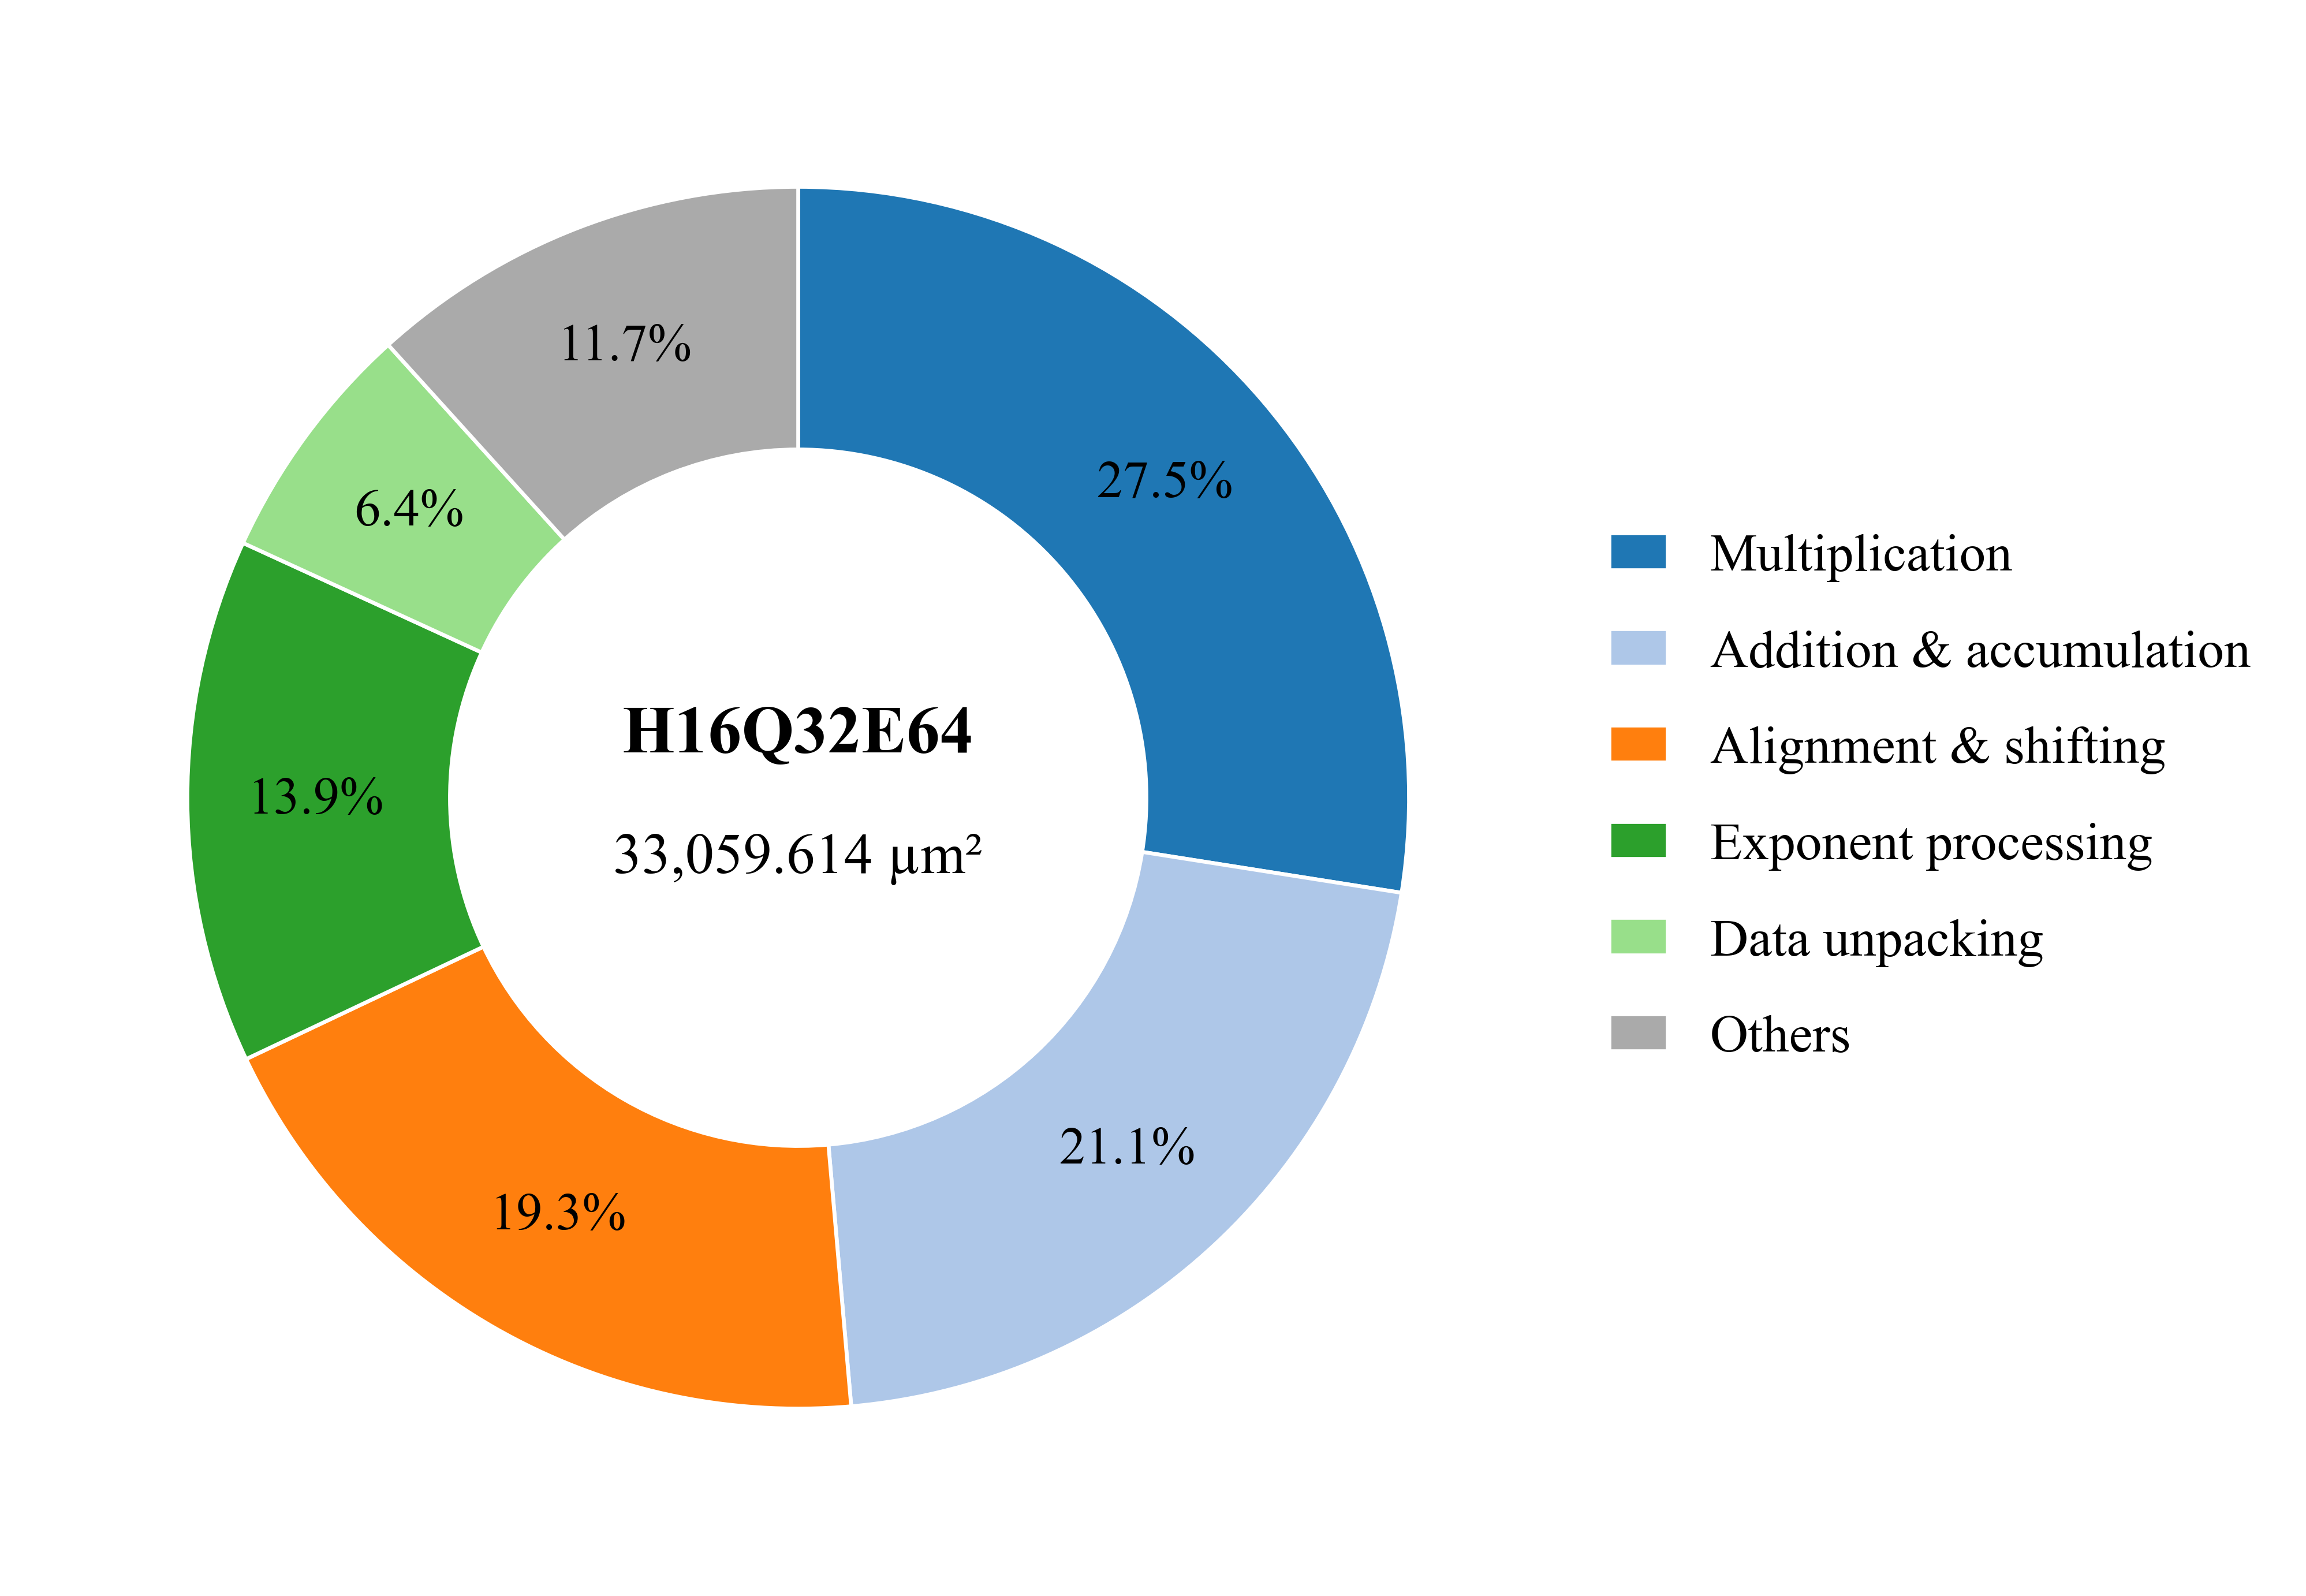
\includegraphics[scale=0.4]{H16Q32E64_area_pie.png}
\caption{Functional area shares of H16Q32E64, including associated registers; denominator: complete DP area.}
\label{fig:full_area_breakdown}
\end{figure}

\subsection{低精度扩展与阵列组织}
\label{sec:kn_evaluation}

\textbf{专用化提高增量算力效率。} 图~\ref{fig:pe_costs_compact} 中，$1:2:8$ 相比 F 增加 34.30\% 面积，将 MXFP4 吞吐提高一倍，每 MAC 能耗降低 23.94\%；$1:2:6$ 的对应能耗降幅为 14.41\%。新增 E 通路的功耗增长小于其吞吐增长，但 FP16/MXFP8 功耗仍增加 2.13\%--2.81\%。因此，低精度扩展的主要收益来自目标模式，未增加算力的模式仍承担附加开销。

\begin{figure}[!t]
\centering
\makebox[\columnwidth][l]{\footnotesize (a) Complete-DP area}\par
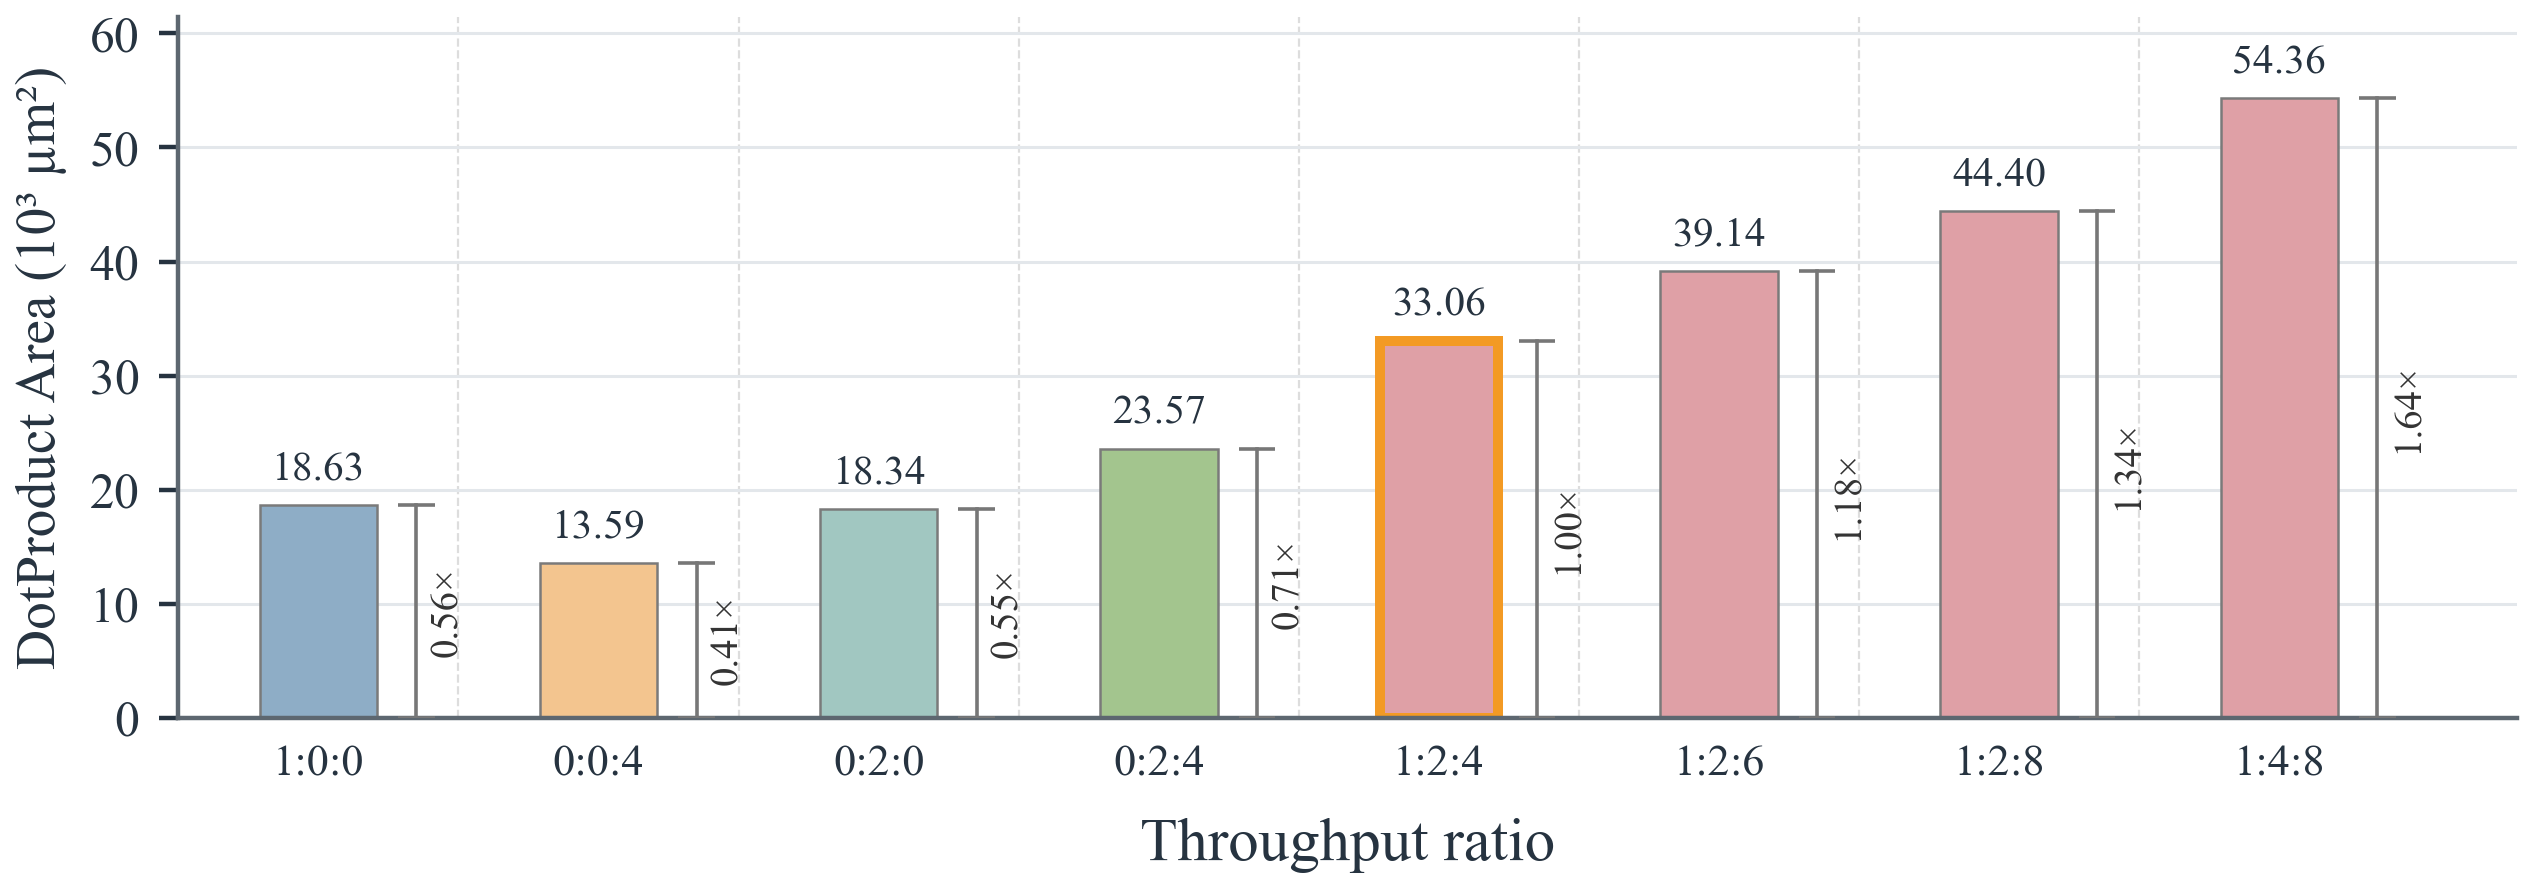
\includegraphics[width=\columnwidth]{selected8_area.png}\par\smallskip
\makebox[\columnwidth][l]{\footnotesize (b) Complete-DP power}\par
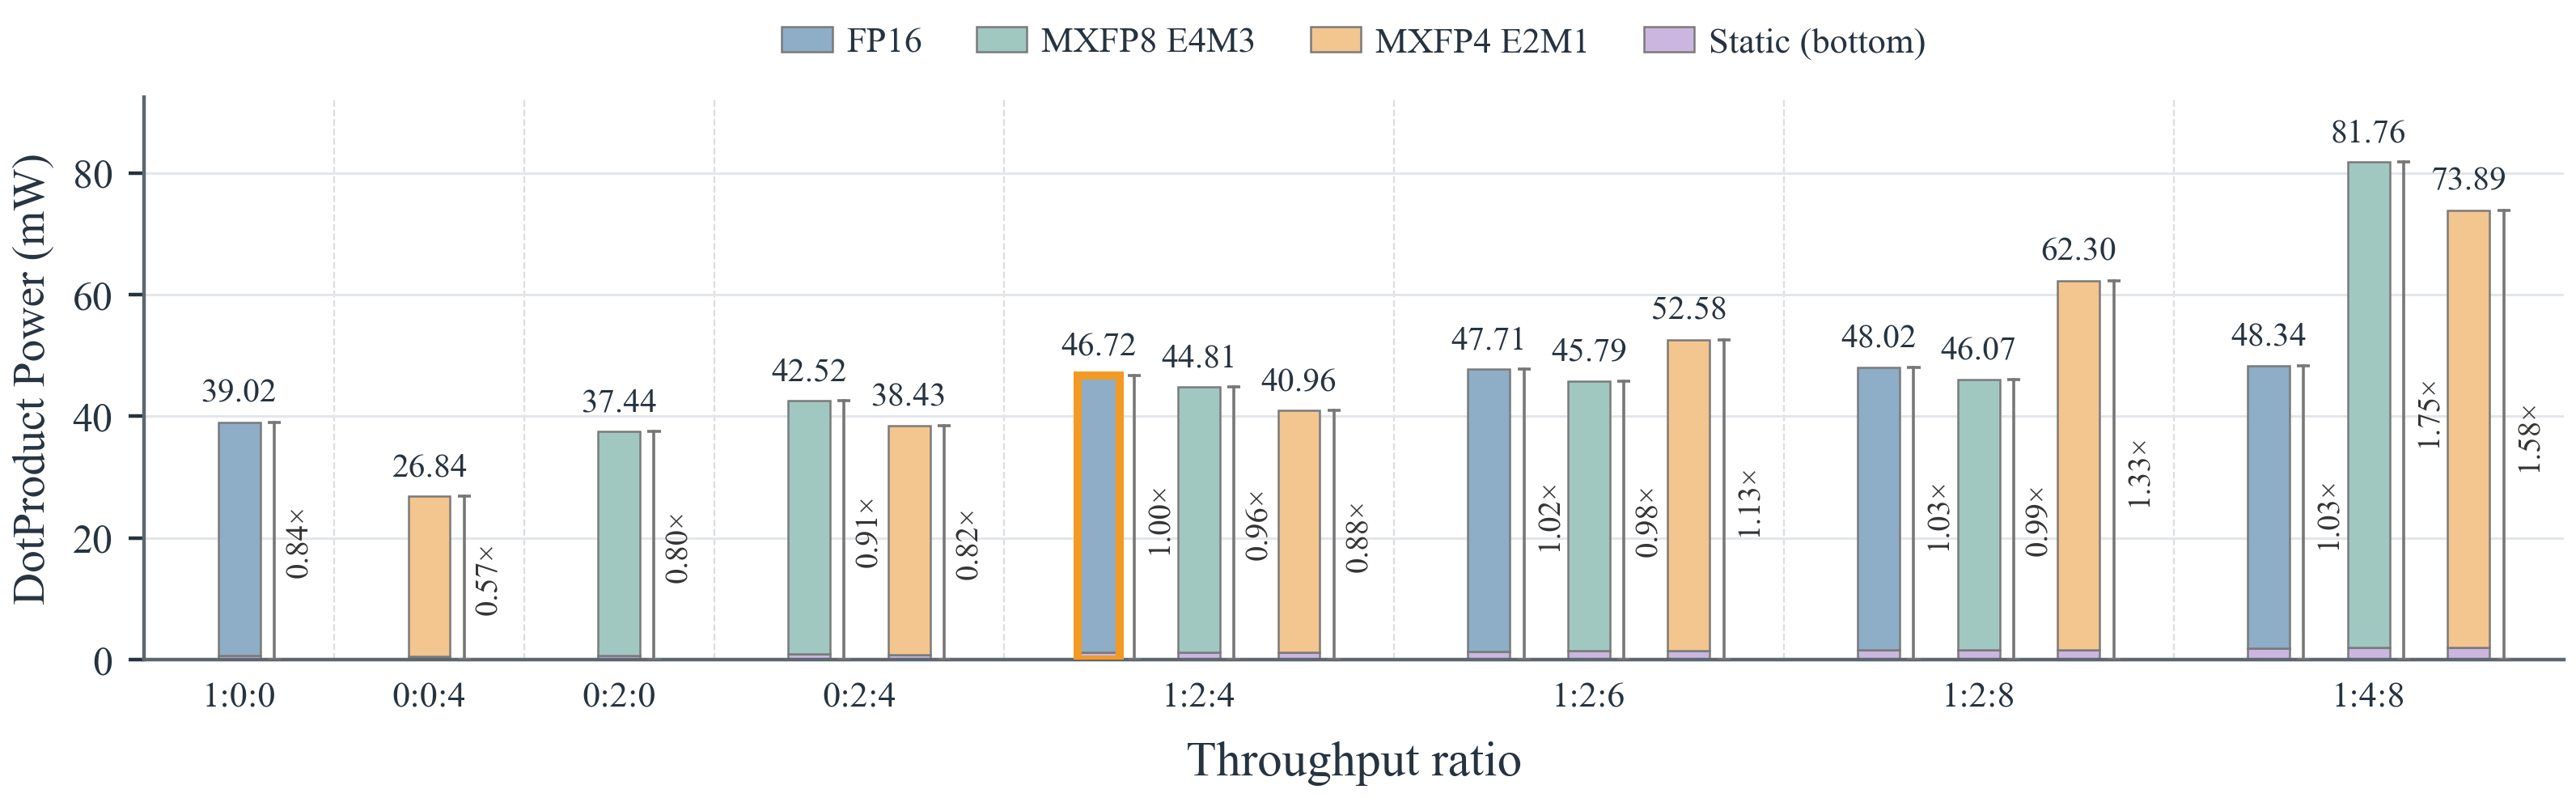
\includegraphics[width=\columnwidth]{selected8_power.png}
\caption{Eight complete-DP costs. Area is relative to F; all power annotations use F--FP16 (46.7175 mW). Power stacks show static and dynamic components for FP16/MXFP8 E4M3/MXFP4 E2M1; zero ratio entries denote unsupported families.}
\label{fig:pe_costs_compact}
\end{figure}

\textbf{共享后端稳定节省面积，能耗收益依赖阵列规模。} 在各精度峰值匹配的 $4\times4$ 基础阵列上，K 组合较 N 组合节省 3.14\%--6.80\% 面积，NVFP4 功耗估计降低 3.79\%--8.03\%（表~\ref{tab:kn_costs}）。扩展到 $16\times4$ 后，K 仍保持面积优势，但 $1:2:6$ 的 NVFP4 功耗估计反而高出 2.01\%。后端共享与新增归约的开销随规模变化，面积收益不能直接外推为能耗收益；在 BF16 模式下，N 关闭附加单元也更有利于抑制功耗。

\begin{table}[t]
\centering
\caption{Estimated K/N costs from a $4\times4$ Full base. Area: mm$^2$; power: W. H/Q/E: BF16/MXFP8 E4M3/NVFP4. N counts active-PE power and inactive leakage.}
\label{tab:kn_costs}
\begingroup\footnotesize\setlength{\tabcolsep}{2.5pt}
\begin{tabular*}{\columnwidth}{@{\extracolsep{\fill}}lcrrrr@{}}\toprule
Ratio & Axis & Area & $P_H$ & $P_Q$ & $P_E$ \\\midrule
$1:2:4$ & K/N & 0.534 & 0.672 & 0.716 & 0.695 \\
$1:2:6$ & K & 0.636 & 0.698 & 0.742 & 0.891 \\
$1:2:6$ & N & 0.656 & 0.679 & 0.721 & 0.926 \\
$1:2:8$ & K & 0.724 & 0.713 & 0.757 & 1.058 \\
$1:2:8$ & N & 0.777 & 0.683 & 0.725 & 1.150 \\
$1:4:8$ & K & 0.883 & 0.718 & 1.306 & 1.238 \\
$1:4:8$ & N & 0.937 & 0.688 & 1.397 & 1.340 \\
\bottomrule
\end{tabular*}\endgroup
\end{table}

\textbf{带宽取舍取决于输出驻留。} 设基础输出形状为 $M\times N$，低精度算力扩展 $r$ 倍，单路输入向量含尺度共 $w$ bit。两方案沿列复用 A、沿行复用 B，每 $\tau$ 次发射交换一次 FP32 C/D。以每次发射的 bit 数计，阵列与本地缓冲间的带宽差为
\begin{equation}
B_N-B_K=(r-1)M\left(\frac{64N}{\tau}-w\right).
\label{eq:kn_bandwidth_difference}
\end{equation}
N 扩列增加 A 的复用，却产生更多独立 C/D 输出；K 扩展减少输出流量，但需要更宽的输入。输出回写频繁时更有利于 K，较长驻留则增强 N 的输入复用收益，与数据流对存储访问成本的影响一致~\cite{timeloop2019}。

按算力密度与单位计算能耗进行 Pareto 比较~\cite{paretomac2025}，四种代表配比在 BF16、MXFP8 和 NVFP4 下的最优者分别为 $1:2:4$、$1:4:8$ 和 $1:2:8$。单精度最优配置并不统一，混合负载的选择还取决于各精度工作量及整核部署成本。

% !TeX root = ../main.tex
\subsection{整核面积约束下的算力分配}
\label{sec:k4_area}

采用 $16\times16$ 阵列，比较四种 $K$ 扩展配比在相同整核面积预算下的部署。H/Q/E 分别以 BF16、MXFP8 E4M3 和 MXFP4 E2M1 为代表格式。华为的 12\,nm RTL 评估中，Cube 簇占 AI Core 面积的 32.7\%，其中计算切片约占 80\%~\cite{luo2024hifloat8area}。据此将基准 DP 阵列的面积占比近似为 $\alpha=0.30$，并采用完整 Ascend 950 架构的 36 个 Cube 单元作为基准数量 $N_0$~\cite{huawei950}。两项数据用于构造等效面积预算，不对应 950 的实际工艺或 die 面积。

令配比 $j$ 的单 DP 面积为 $a_j$，阵列面积 $A_{T,j}=256a_j$，下标 0 表示 $1:2:4$。基准整核面积、固定外围面积及总预算为
\begin{equation}
A_{C,0}=\frac{A_{T,0}}{\alpha},\quad
A_O=A_{C,0}-A_{T,0},\quad
A_{\mathrm{bud}}=N_0A_{C,0}.
\label{eq:k4_area_definition}
\end{equation}
固定每核外围面积 $A_O$，在 $A_{\mathrm{bud}}=405.57$\,mm$^2$ 内重新部署完整核心：
\begin{equation}
n_j=\left\lfloor\frac{A_{\mathrm{bud}}}{A_O+A_{T,j}}\right\rfloor.
\label{eq:core_area_budget}
\end{equation}
设 $m_{j,f}$ 和 $p_{j,f}$ 为单 DP 在精度 $f$ 下的每周期 MAC 数与活动功耗，频率为 $\nu$。按一次 MAC 等于两个 FLOP，部署后的总算力与 DP 功耗为
\begin{equation}
C_{j,f}=2\nu\,256n_jm_{j,f},\qquad
P_{j,f}=256n_jp_{j,f}.
\label{eq:k4_capacity_power}
\end{equation}

表~\ref{tab:k4_absolute} 表明，低精度扩展同时改变单核能力与可部署核心数。$1:4:8$ 将核心数从 36 减至 29，Q 总算力仍提高 61.11\%，H 总算力却下降 19.44\%。因此，低精度加速必须补偿高精度阶段因核心减少而增加的时间，单 DP 峰值不足以判断整核收益。

\begin{table}[!t]
\centering
\caption{Area-constrained N12 deployment. $A_C$: core area (mm$^2$); $C$: TFLOP/s; $P$: DP-only power (W).}
\label{tab:k4_absolute}
\begingroup\footnotesize\setlength{\tabcolsep}{3pt}
% Generated by scripts/reproduce.py.
\begin{tabular*}{\linewidth}{@{\extracolsep{\fill}}lrrcc@{}}\toprule
Ratio & $A_C$ & $n$ & $C_H/C_Q/C_E$ & $P_H/P_Q/P_E$ \\\midrule
$1:2:4$ & 11.266 & 36 & 415.8/831.7/1663.3 & 233.1/232.5/223.3 \\
$1:2:6$ & 12.053 & 33 & 381.2/762.3/2287.0 & 219.3/218.7/260.3 \\
$1:2:8$ & 12.567 & 32 & 369.6/739.2/2957.0 & 210.8/210.1/297.3 \\
$1:4:8$ & 13.615 & 29 & 335.0/1339.9/2679.8 & 192.7/320.1/301.3 \\
\bottomrule\end{tabular*}

\endgroup
\end{table}

\subsection{混合精度负载的性能与能耗}
\label{sec:k4_simplex}

令 $F=\sum_f F_f$ 为 H/Q/E 有效 GEMM 总计算量，$x_f=F_f/F$ 且 $\sum_f x_f=1$。三角坐标表示 FLOP 占比。各精度阶段依次使用全部核心并充分利用对应算力时，计算时间、有效算力和 DP 能耗为
\begin{align}
T_j&=F\sum_f\frac{x_f}{C_{j,f}},&
C_{\mathrm{eff},j}&=\frac{F}{T_j},
\label{eq:k4_time}\\
\mathcal E_j&=F\sum_f x_f\frac{P_{j,f}}{C_{j,f}},&
\varepsilon_{j,f}&=\frac{P_{j,f}}{C_{j,f}}.
\label{eq:k4_energy}
\end{align}
能耗由各精度的计算时间乘对应活动功耗累加，仅计 DP 计算。核心数在单位 FLOP 能耗 $\varepsilon_{j,f}=p_{j,f}/(2\nu m_{j,f})$ 中抵消：增加核心缩短执行时间，却不改变该模型下的单位工作能耗。因此，面积约束通过可部署算力影响时间，而能耗取决于各精度的功耗--吞吐比，两种目标对应不同的最优配比区域。

$T_j$ 和 $\mathcal E_j$ 均为负载组成 $\boldsymbol x$ 的线性函数，候选成本相等处构成分区边界。以 1 个百分点为步长覆盖 5,151 种组成，图~\ref{fig:k4_time_prefill} 分别给出最大有效算力和最低能耗区域，表~\ref{tab:k4_regions} 给出 E 为 MXFP4 时的区域面积占比。

NVFP4 与 MXFP4 共用 E 算力，但单位能耗不同。令 $\rho$ 为 E 工作中 NVFP4 的比例，则 $\varepsilon_{j,E}=(1-\rho)\varepsilon_{j,\mathrm{MX}}+\rho\varepsilon_{j,\mathrm{NV}}$。能耗图的实色区域在两种编码间保持同一最优配比，斜线区域的选择依赖 $\rho$；各模型点按实际编码组成计算能耗。

\begin{figure}[!t]
\centering
\begin{minipage}[t]{0.49\columnwidth}
\centering
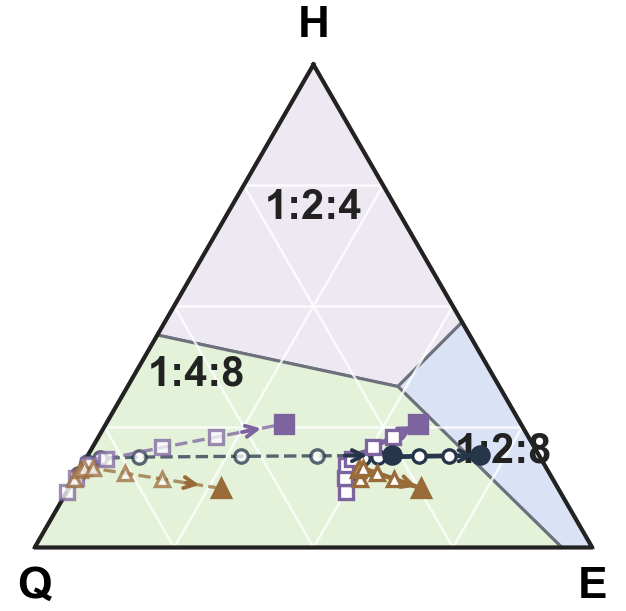
\includegraphics[width=\linewidth]{k4_n12_prefill_time.png}
{\footnotesize (a) Effective throughput\par}
\end{minipage}\hfill
\begin{minipage}[t]{0.49\columnwidth}
\centering
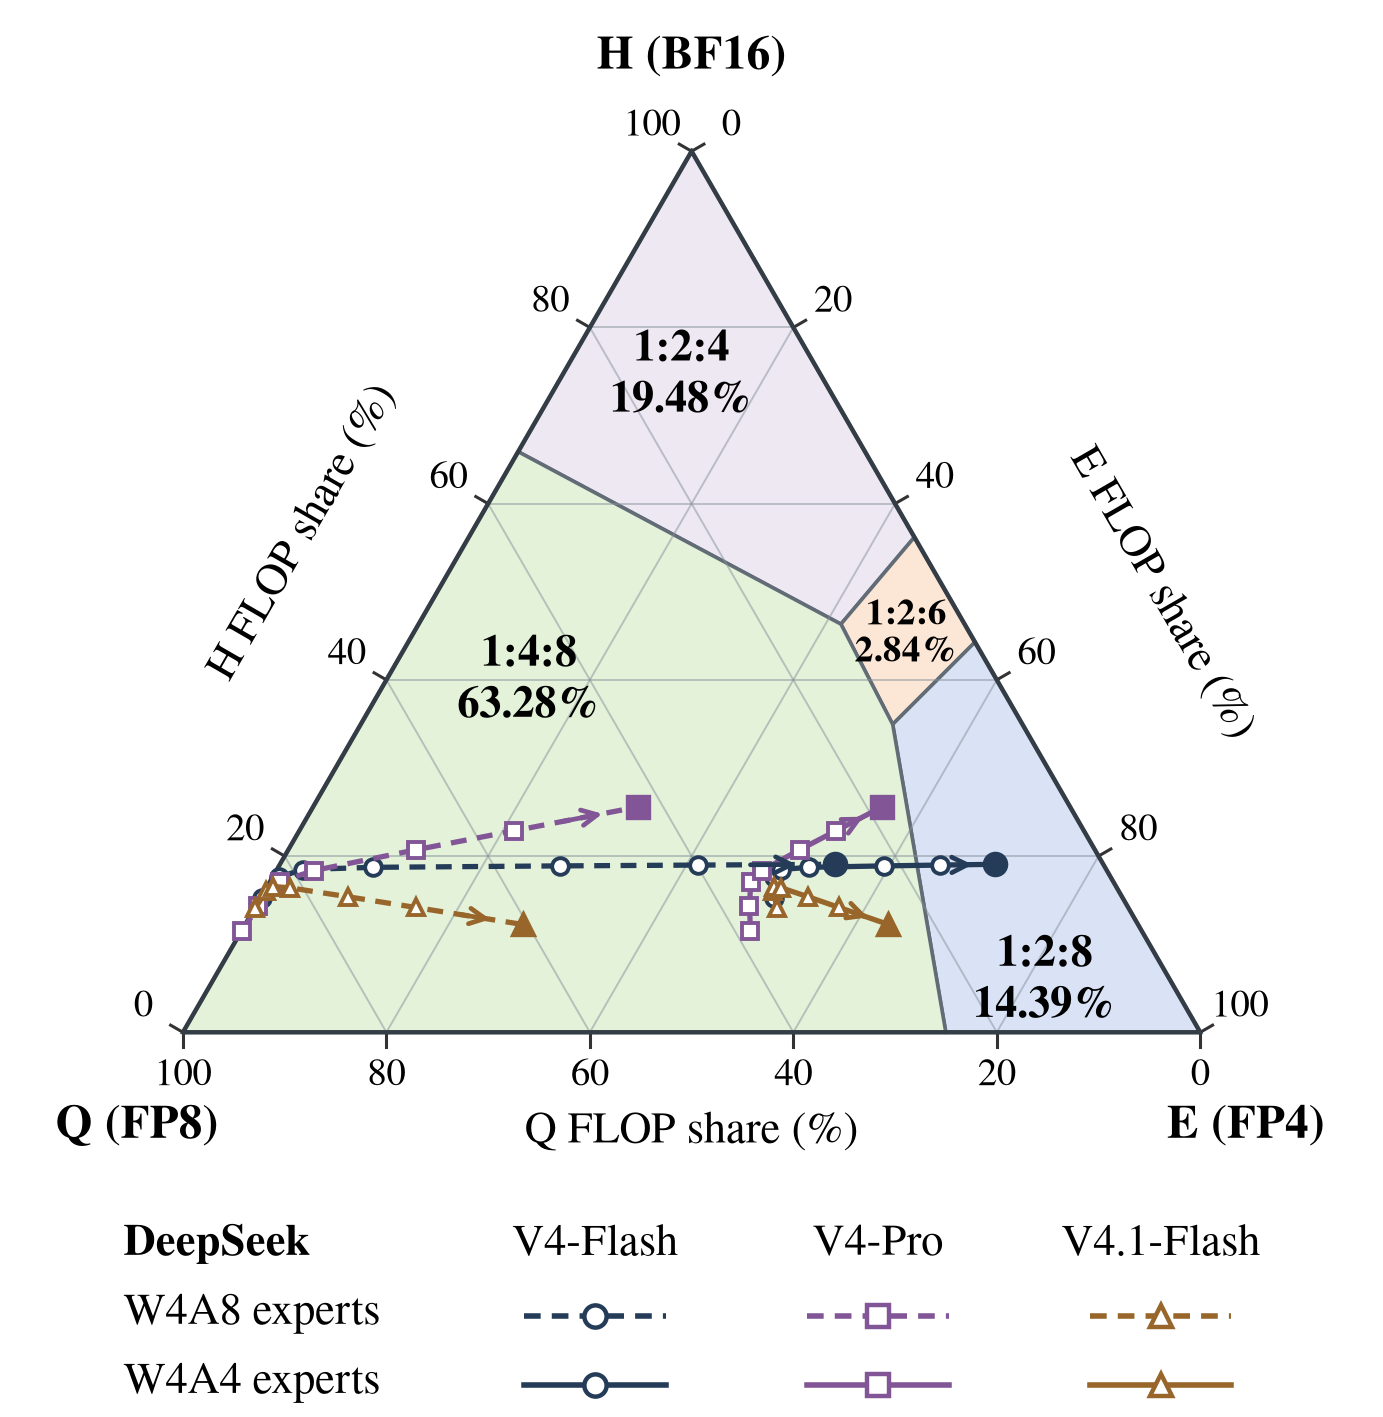
\includegraphics[width=\linewidth]{k4_n12_prefill_energy.png}
{\footnotesize (b) DP compute energy\par}
\end{minipage}
\par\smallskip
{\scriptsize $\circ$ V4-Flash\quad $\square$ V4-Pro\quad $\triangle$ V4.1-Flash\par}
{\scriptsize Dashed: W4A8 experts\quad Solid: NVFP4 W4A4 experts\par}
\caption{Area-constrained ratio selection and prefill trajectories. H/Q/E denote BF16/FP8/FP4 FLOP shares. Arrows follow 1K, 4K, 16K, 64K, 256K, 512K and 1M contexts; filled markers denote 1M. In (b), hatching marks regions whose optimum depends on the MXFP4/NVFP4 mix.}
\label{fig:k4_time_prefill}
\label{fig:k4_energy_prefill}
\end{figure}

\begin{table}[!t]
\centering
\caption{Optimal-region fractions with MXFP4 as E. Energy fractions are unchanged by integer core deployment.}
\label{tab:k4_regions}
\begingroup\footnotesize\setlength{\tabcolsep}{2pt}
% Generated by scripts/reproduce.py.
\begin{tabular*}{\linewidth}{@{\extracolsep{\fill}}lrrr@{}}\toprule
Ratio & Time (cont.) & Time (int.) & DP energy \\\midrule
$1:2:4$ & 31.63\% & 36.85\% & 8.51\% \\
$1:2:6$ & 1.44\% & 0.00\% & 0.00\% \\
$1:2:8$ & 8.44\% & 10.30\% & 23.75\% \\
$1:4:8$ & 58.49\% & 52.85\% & 67.74\% \\
\bottomrule\end{tabular*}

\endgroup
\end{table}

H 密集负载偏向 $1:2:4$，E 密集负载偏向 $1:2:8$，$1:4:8$ 则覆盖较广的混合精度区域。整数部署使 $1:2:6$ 的时间最优区域从连续面积分配下的 1.44\% 消失；其三种精度的单位 FLOP 能耗又均高于 $1:2:8$，因而也不存在能耗最优区域。中间配比并不必然提供独立的负载优势，核心部署粒度和精度相关能效比峰值配比的间隔更具决定性。

\subsection{模型精度需求与配比选择}
\label{sec:k4_prefill}

依据 DeepSeek 的官方配置、推理代码和技术报告~\cite{deepseekv4,deepseekv4flashsource,deepseekv4prosource,deepseekv41source}，分析 V4-Flash、V4-Pro 和 V4.1-Flash 在 batch=1、1K--1M 上下文下的纯文本冷启动 prefill。参考映射将原生 MXFP4 索引点积归入 E，W4A8 路由专家和 FP8 投影归入 Q，BF16 注意力与分组输出投影归入 H。进一步依据已发布的 NVFP4 量化配置~\cite{nvidia2026v4flashnvfp4,nvidia2026v4pronvfp4,nvidia2026deepseeknvfp4}，将路由专家的三个 GEMM 全部映射为 NVFP4 W4A4，其余计算保持不变。同一上下文下，专家量化使 H 不变、Q 向 E 转移。

GEMM 按 $2MNK$ 计数，MoE 仅计激活专家，注意力与索引器遵循因果、窗口、压缩及 top-$k$ 约束。V4.1 进一步计入 CED 的 encoder prefill、decoder 缓存构建和有限窗口重放，并考虑跨层索引复用~\cite{deepseekv41source}。H/Q/E 覆盖所统计 GEMM FLOP 的 97.11\%--99.37\%，其余为 FP32。两个图均叠加参考 W4A8 与专家 W4A4 的上下文轨迹，每种映射包含 21 个点。

\begin{table}[!t]
\centering
\caption{Reference W4A8 prefill endpoints. H/Q/E shares are normalized over useful GEMM FLOPs. Speedup and DP energy reduction $\Delta E$ compare $1:4:8$ against $1:2:4$.}
\label{tab:k4_prefill_points}
\begingroup\footnotesize\setlength{\tabcolsep}{4pt}
% Generated by scripts/reproduce.py.
\begin{tabular*}{\linewidth}{@{\extracolsep{\fill}}llcrr@{}}\toprule
Model & $S$ & $x_H/x_Q/x_E$ (\%) & Speedup & $\Delta E$ (\%) \\\midrule
V4-Flash & 1K & 15.25/84.58/0.17 & 1.274 & 6.77 \\
V4-Flash & 1M & 19.07/26.39/54.55 & 1.138 & 3.93 \\
V4-Pro & 1K & 11.54/88.40/0.06 & 1.335 & 7.49 \\
V4-Pro & 1M & 25.59/42.45/31.96 & 1.098 & 3.75 \\
V4.1-Flash & 1K & 14.08/85.86/0.06 & 1.292 & 7.00 \\
V4.1-Flash & 1M & 12.24/60.49/27.27 & 1.291 & 6.65 \\
\bottomrule\end{tabular*}

\endgroup
\end{table}

\textbf{参考 W4A8 负载受益于 FP8 算力扩展。} 三个模型在短上下文下均以 FP8 计算为主，参考映射的全部采样点在两种目标下均选择 $1:4:8$。V4-Flash 的 E 占比随上下文增长，在 1M 时达到 54.55\%，但 Q 仍占 26.39\%；扩展 FP8 通路的收益足以抵消其相对 $1:2:8$ 的 FP4 算力损失。FP4 工作量占多数尚不足以改变最优配比。

\textbf{上下文增长的影响取决于模型结构。} 参考映射中，V4-Pro 的 H 占比在 1M 时增至 25.59\%，$1:4:8$ 的加速比由 1.335 降至 1.098。V4.1-Flash 则因 CED 与索引复用形成不同轨迹：1M 时 Q 仍占 60.49\%，H 降至 12.24\%，保持 1.291 倍加速和 10.47\% 的 DP 节能（表~\ref{tab:k4_prefill_points}）。高精度注意力、FP8 投影与 FP4 索引计算的相对增长共同决定扩展收益。

\textbf{专家 W4A4 已推动配比转向 $1:2:8$。} 量化后，V4-Flash 的 E 占比由 1K 的 50.52\% 增至 1M 的 70.26\%，Q 则降至 10.68\%。在采样点中，512K 时能耗最优先转向 $1:2:8$，1M 时吞吐也完成切换。V4-Pro 与 V4.1-Flash 在 1M 时仍分别保留 18.46\% 和 24.54\% 的 Q 工作，均选择 $1:4:8$。因此，FP4 专家量化与上下文增长可共同推动配比变化，但剩余 FP8 需求使这种转移具有模型差异。



% !TeX root = ../main.tex
\section{面积约束下的算力配比设计空间探索}
\label{sec:workload}

本节以四种 DP 的面积、原生点积长度和活动功耗为输入，在统一整核面积预算下，分别求解混合精度负载的延迟与计算能耗最优配比。分析对象是计算资源充分利用时的 GEMM 服务时间；带宽、边界利用率和调度损失尚未计入，因此结果用于刻画配比的计算侧收益。

\subsection{从单 DP 成本到整核部署}
\label{sec:k4_area}

每个 AI 核心采用 $m=n=16$ 的 DP 阵列。参考计算单元面积构成研究~\cite{luo2024hifloat8area}及公开核心数量~\cite{huawei950}，取基准阵列面积占比 $\alpha=0.30$、基准核心数 $N_0=36$，构造等效预算；该预算不代表实际芯片面积。

令配比 $j$ 的单 DP 面积为 $a_j$，阵列面积为 $A_{T,j}=mn a_j$，下标 0 表示 $1:2:4$。基准整核面积、固定外围面积和总预算为
\begin{equation}
A_{C,0}=\frac{A_{T,0}}{\alpha},\quad
A_O=A_{C,0}-A_{T,0},\quad
A_{\mathrm{bud}}=N_0A_{C,0}.
\label{eq:k4_area_definition}
\end{equation}
保持每核外围面积 $A_O$ 不变，在 $A_{\mathrm{bud}}=496.59$\,mm$^2$ 内部署的完整核心数为
\begin{equation}
n_j=\left\lfloor\frac{A_{\mathrm{bud}}}{A_O+A_{T,j}}\right\rfloor.
\label{eq:core_area_budget}
\end{equation}
以 $p\in\{H,Q,E\}$ 表示精度，$K_{j,p}$ 为单 DP 的原生点积长度，$p_{j,p}$ 为第~\ref{sec:evaluation} 节测得的模式功耗。在 $f=1$\,GHz 下，总峰值算力与 DP 活动功耗为
\begin{equation}
C_{j,p}=2fmn n_jK_{j,p},\qquad
P_{j,p}=mn n_jp_{j,p}.
\label{eq:k4_capacity_power}
\end{equation}

\begin{table}[t]
\centering
\caption{面积预算下的部署结果。$A_C$：整核面积（mm$^2$）；$C$：峰值算力（TFLOP/s）；$P$：仅 DP 的活动功耗（W）。}
\label{tab:k4_absolute}
\begingroup\footnotesize\setlength{\tabcolsep}{3pt}
% Generated by scripts/reproduce.py.
\begin{tabular*}{\linewidth}{@{\extracolsep{\fill}}lrrcc@{}}\toprule
Ratio & $A_C$ & $n$ & $C_H/C_Q/C_E$ & $P_H/P_Q/P_E$ \\\midrule
$1:2:4$ & 11.266 & 36 & 415.8/831.7/1663.3 & 233.1/232.5/223.3 \\
$1:2:6$ & 12.053 & 33 & 381.2/762.3/2287.0 & 219.3/218.7/260.3 \\
$1:2:8$ & 12.567 & 32 & 369.6/739.2/2957.0 & 210.8/210.1/297.3 \\
$1:4:8$ & 13.615 & 29 & 335.0/1339.9/2679.8 & 192.7/320.1/301.3 \\
\bottomrule\end{tabular*}

\endgroup
\end{table}

四种配比分别可部署 36、34、32、29 个核心（表~\ref{tab:k4_absolute}）。$1:2:8$ 与 $1:4:8$ 的单 DP E 吞吐相同，但前者可部署更多核心，获得更高 E 总算力；后者则以部署密度下降换取更高 Q 总算力。单 DP 的吞吐优势因此不能直接等同于固定面积下的系统收益。

\subsection{混合精度负载与优势区域}
\label{sec:k4_simplex}

令 $F_p$ 为精度 $p$ 的有效 GEMM 工作量，$F=\sum_pF_p$，$x_p=F_p/F$，且 $\sum_p x_p=1$。假设各精度阶段顺序执行并充分利用全部核心，计算延迟与 DP 能耗分别为
\begin{align}
T_j&=F\sum_p\frac{x_p}{C_{j,p}},
\label{eq:k4_time}\\
\mathcal E_j&=F\sum_p x_p\frac{P_{j,p}}{C_{j,p}}.
\label{eq:k4_energy}
\end{align}
面积预算覆盖整核，而能耗只包含 DP 计算部分，未加入外围、存储和数据传输。本文分别最小化 $T_j$ 与 $\mathcal E_j$，不将两者合并为单一评分。

在 H/Q/E 三角域内，以 1 个百分点的间隔扫描 5,151 种工作量组成。固定 $F$ 时，两项目标均为 $\boldsymbol x$ 的线性函数，任意两种配比的等成本条件给出直线边界。图~\ref{fig:k4_time_prefill} 标注最优区域的几何面积占比，不代表应用出现概率。

\begin{figure}[t]
\centering
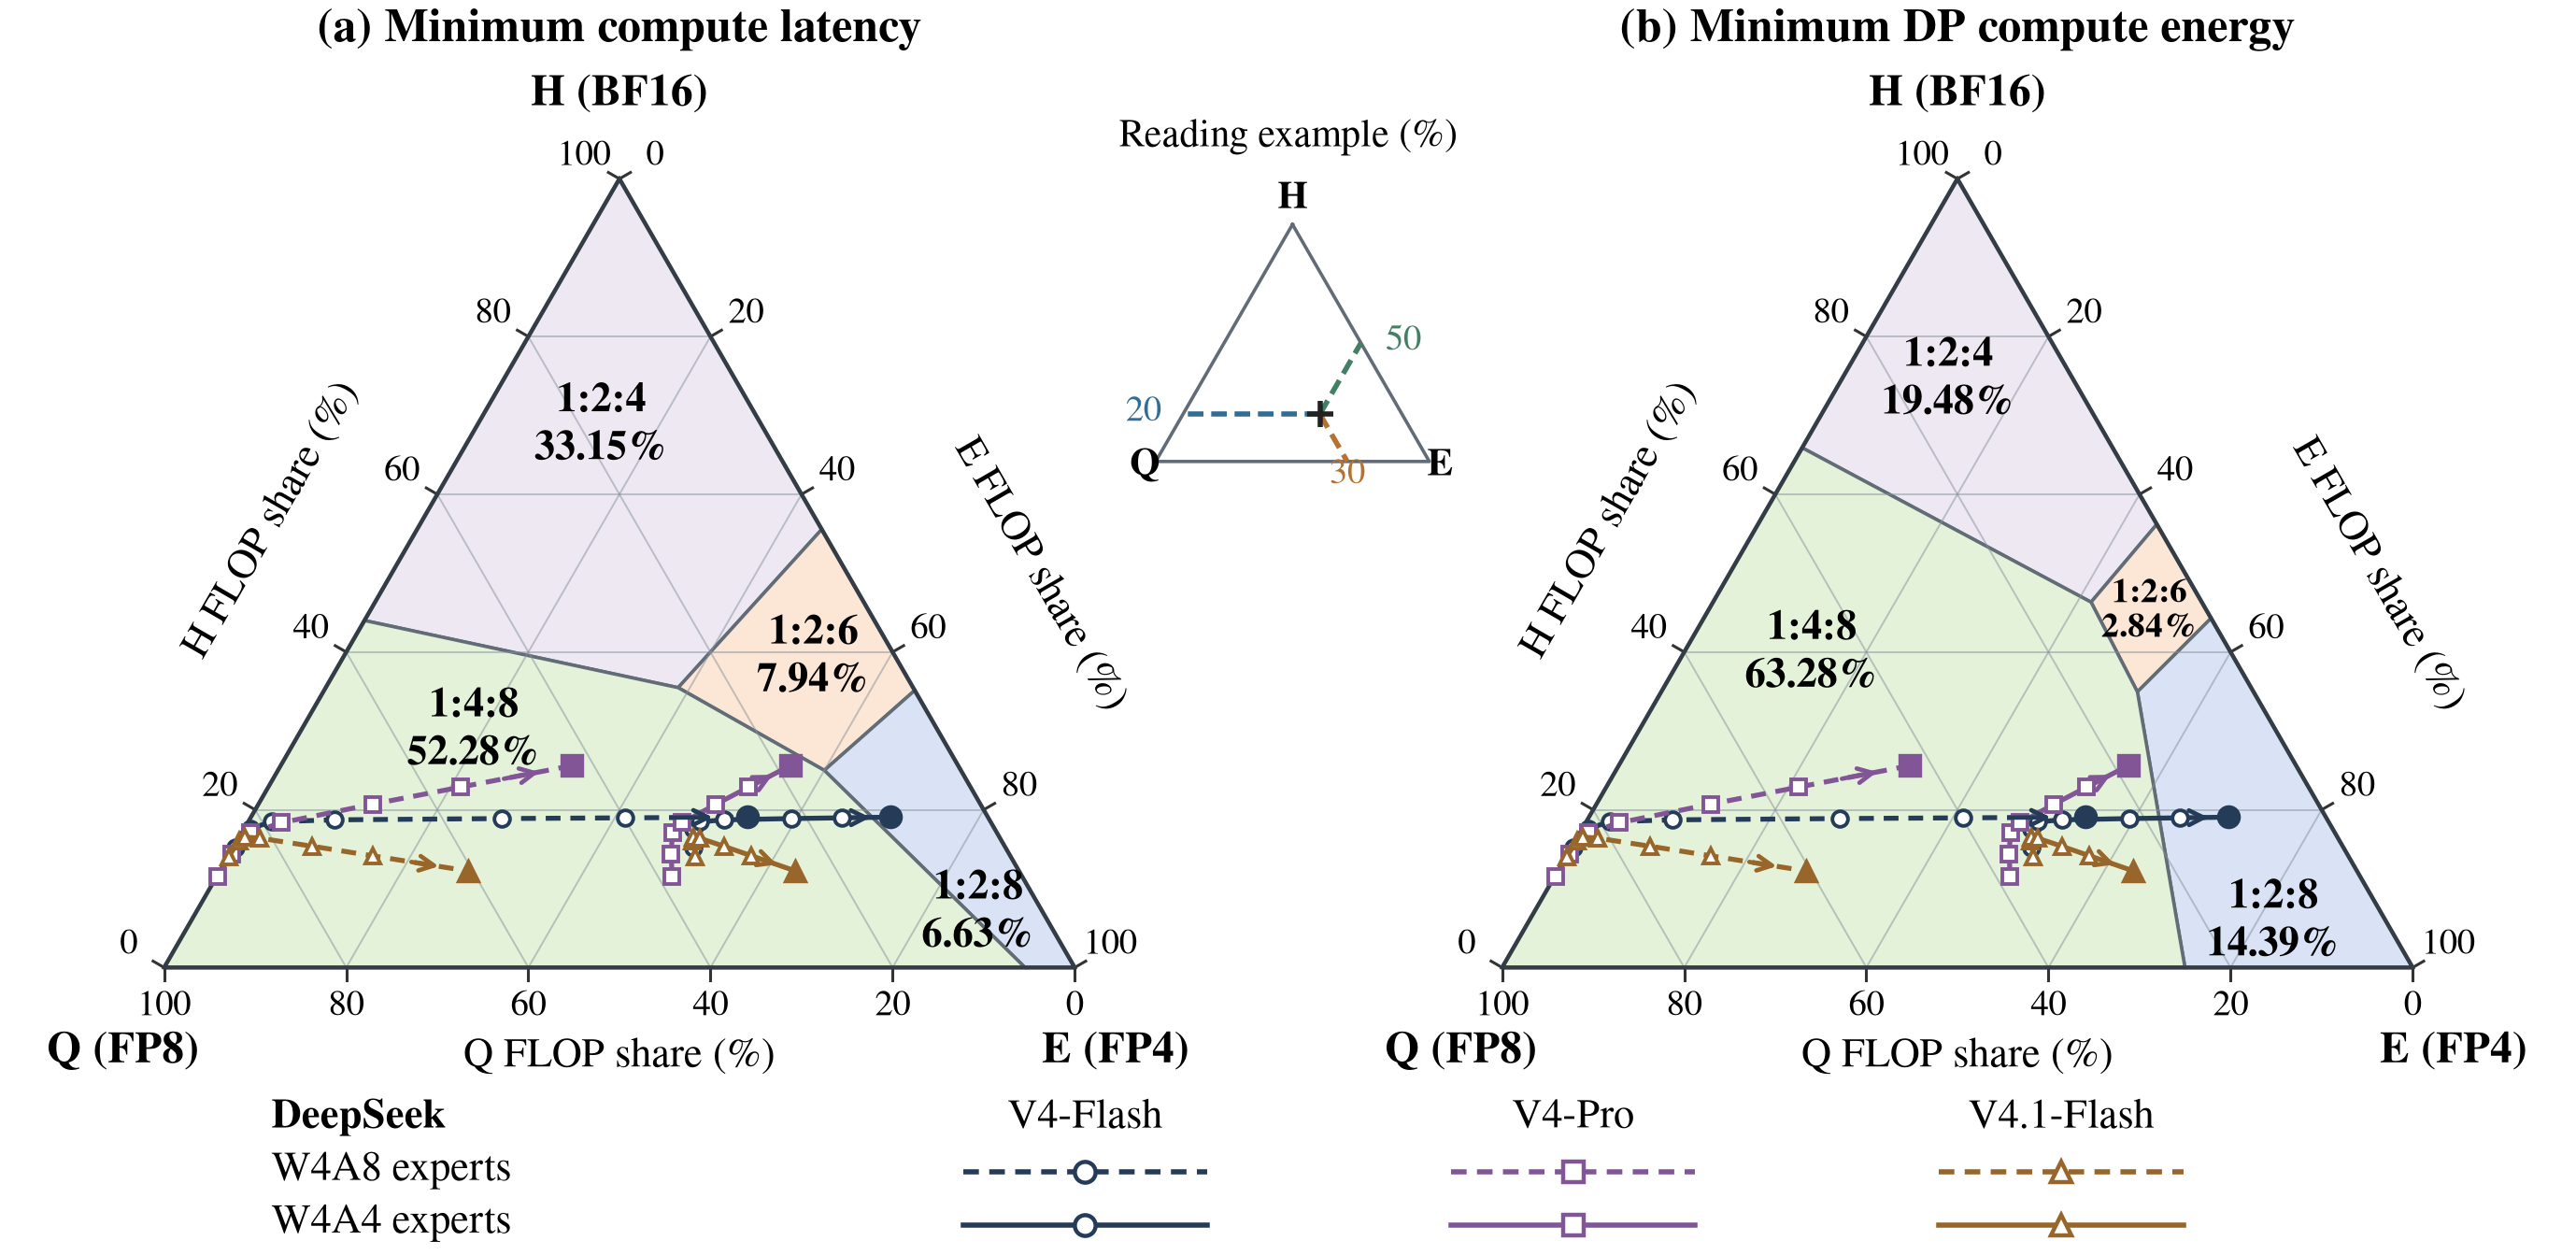
\includegraphics[width=\columnwidth]{k4_n12_prefill_comparison.png}
\caption{等面积下的配比选择：(a) 计算延迟；(b) DP 计算能耗。区域标注为最优配比及其几何占比，小图示例为 H/Q/E=20\%/30\%/50\%。轨迹由 DeepSeek 模型结构导出，虚线为专家 W4A8，实线为专家 W4A4 迁移场景，其余计算不变。箭头依次对应 1K、4K、16K、64K、256K、512K、1M 上下文，实心标记为 1M。NVFP4 能耗使用 MXFP4 功耗代理。}
\label{fig:k4_time_prefill}
\end{figure}

H、E、Q 密集区域分别倾向于 $1:2:4$、$1:2:8$ 和 $1:4:8$；$1:2:6$ 在 H/E 混合且 Q 较少时，以较小面积增量平衡 E 加速与 H 吞吐损失。延迟由各阶段的 $F_p/C_{j,p}$ 决定。单位 FLOP 能耗为 $P_{j,p}/C_{j,p}=p_{j,p}/(2fK_{j,p})$，在当前模型中与核心数抵消，因此延迟与能耗的优势区域不完全重合。

\textbf{观察二：面积约束改变了峰值配比的收益顺序。} 增配低精度通路会减少核心数量，H 阶段无法从单核增配中获益；只有被加速阶段节省的时间足以补偿其余阶段的吞吐损失时，增配才降低总延迟。

\subsection{模型工作量与执行精度映射}
\label{sec:workload_extraction}

工作量统计以 GEMM 算子而非参数存储量为单位。依据固定模型配置和计算规则，确定各投影、注意力及专家算子的 $M,N,K$ 和调用次数，再按 $2MNK$ 汇总。MoE 只计实际激活专家；稀疏或压缩注意力按其有效计算结构统计。每个算子依据权重、激活及执行方式归入 H/Q/E，其他精度单独保留，不强行映射。例如，专家权重虽以 4 位存储，W4A8 执行仍归入 Q；仅当该算子采用 W4A4 执行时才归入 E。

当前采用固定配置与模型特定规则进行可复算的静态分析，后续将结合自动化算子提取与执行轨迹，核验实际内核精度并扩展模型覆盖。
% 后续实验：补入固定版本的 DeepSeek-V3.2；可选完整 DeepSeek-R1。
% 两个实际专家量化版本须分别核验 checkpoint、执行后端与算子覆盖，
% 不能将下述 W4A4 迁移场景直接称为两个已验证量化模型。

\subsection{DeepSeek 负载与低精度迁移}
\label{sec:k4_prefill}

依据官方配置~\cite{deepseekv4,deepseekv4flashsource,deepseekv4prosource,deepseekv41source}，统计 V4-Flash、V4-Pro、V4.1-Flash 在 batch=1、1K--1M 七种上下文下的冷启动 prefill，纳入稀疏/压缩注意力以及 V4.1 的 CED 与索引复用。BF16 注意力与分组输出投影归入 H，W4A8 专家计算和 FP8 投影归入 Q，MXFP4 索引点积归入 E。另构造仅将路由专家改为 NVFP4 W4A4 的迁移场景，其余计算保持不变。两组映射各含 21 个负载点，H/Q/E 覆盖其 GEMM 工作量的 97.11\%--99.37\%；图中的占比仅在这三类内归一化。

全部 W4A8 采样点均以 $1:4:8$ 的计算延迟和 DP 能耗最低。专家迁移至 W4A4 后，V4-Flash 在 512K 的能耗最优配比、1M 的延迟最优配比转为 $1:2:8$，另两模型至 1M 仍选择 $1:4:8$。在 V4-Flash 的 1M 点，$1:2:8$ 相对 $1:4:8$ 的延迟与估计能耗优势仅为 1.45\% 和 2.03\%，说明该点靠近配比边界，不宜据此推断普遍优势。

可进一步用受控迁移描述未来需求：设现有 Q 工作量中有比例 $\lambda$ 转为 E，算子形状与总工作量保持不变，则
\begin{equation}
\boldsymbol x(\lambda)=
\bigl(x_H,(1-\lambda)x_Q,x_E+\lambda x_Q\bigr),\quad 0\le\lambda\le1.
\label{eq:precision_migration}
\end{equation}
将其代入式~\eqref{eq:k4_time} 和式~\eqref{eq:k4_energy} 可分别求得延迟、能耗的配比切换条件。该路径用于隔离执行精度变化的影响，不代表量化后的模型精度已得到验证。

\textbf{观察三：当前与未来的较优配比取决于执行精度迁移。} 采样的 DeepSeek W4A8 结构保留较多 Q 工作量，使 $1:4:8$ 受益；若更多 Q 计算能够转为 E，$1:2:8$ 的部署密度和 E 总算力优势将更有价值。实际切换点同时取决于残留 H/Q 工作量，不能仅凭采用 FP4 权重判断。

模型采用统一 Qwen 活动功耗代理 DeepSeek，并以 MXFP4 代理 NVFP4，未计入格式转换、供数开销及外围面积增长。完整推理收益仍需通过执行轨迹、带宽约束与跨负载功耗校准验证。


% !TeX root = ../main.tex
\section{结论}
\label{sec:conclusion}

DP-Puzzle 以组合式点积微架构提供可实现候选，将同工况面积、逐模式功耗与混合精度工作量纳入算力配比 DSE。结果表明，算力与硬件成本不等比例增长，面积约束下的部署密度进一步影响配比收益。当前 DeepSeek prefill 的 W4A8 采样点倾向于 $1:4:8$；更多计算转向 E 时，$1:2:8$ 可在部分场景中受益，边界取决于残留 H/Q 工作量。后续通过自动化工作量提取、跨版本对照及带宽与功耗校准，验证这些计算侧趋势的系统适用性。


\section*{Content Generated by AI}
本研究使用 OpenAI Codex 辅助 EDA 脚本生成、源码与微架构说明梳理，以及实验建模、数据分析、图表脚本和全文结构与文字草稿的整理。作者对采用的脚本、结果及全部论述承担责任。



\clearpage
\setcounter{DACreferencepage}{\value{page}}
\ifnum\value{DACreferencepage}>7\relax
  \PackageWarningNoLine{DAC2027}{Main text exceeds six pages}%
\fi
\typeout{DAC2027: References start on page \thepage}
\bibliographystyle{IEEEtran}
\bibliography{references/references}

\end{document}
